\documentclass{book}
\title{Notas de clase Cálculo integral \\ UFM \\ SECCIÓN A}
\author{Christiaan Ketelaar \\ Organizado por: David Corzo}
\date{2019-10-09}
%%%%%%%%%%%%%%%%%%%%%%%%%%%%%%%%%%%%%%%%%%%%%%%%%%%%%%%%%%%%%%%%%%%%%%%%%%%%%%%%%%%%%%%%%%%%%%%%%%%%%%%%%%%%%%%%%%%%%%%%%%%%%%%%%%%%%%%%%%%%%%%
\usepackage[margin = 1in]{geometry}
\usepackage{graphicx}
\usepackage{fontenc}
\usepackage{pdfpages}
\usepackage[spanish]{babel}
\usepackage{amsmath}
\usepackage{amsthm}
\usepackage[utf8]{inputenc}
\usepackage{enumitem}
\usepackage{mathtools}
\usepackage{import}
\usepackage{xifthen}
\usepackage{pdfpages}
\usepackage{transparent}
\usepackage{color}
\usepackage{fancyhdr}
\usepackage{lipsum}
\usepackage{sectsty}
\usepackage{titlesec}
\usepackage{calc}
\usepackage{lmodern}
\usepackage{xpatch}
\usepackage{blindtext}
\usepackage{bookmark}
\usepackage{fancyhdr}
\usepackage{xcolor}
\usepackage{tikz}
\usepackage{blindtext}
%%%%%%%%%%%%%%%%%%%%%%%%%%%%%%%%%%%%%%%%%%%%%%%%%%%%%%%%%%%%%%%%%%%%%%%%%%%%%%%%%%%%%%%%%%%%%%%%%%%%%%%%%%%%%%%%%%%%%%%%%%%%%%%%%%%%%%%%%%%%%%%
% Clear the header and footer
\fancyhead{}
\fancyfoot{}
% Set the right side of the footer to be the page number
{\fontfamily{mc}\selectfont
\fancyfoot[L]{\thepage}
\fancypagestyle{plain}{
    \renewcommand{\headrulewidth}{0pt}
    \fancyhf{}
    \fancyfoot[L]{\thepage}
}}

% THIS IS TO CENTER AND DEDICATE A CHAPTER NAME AN ENTIRE PAGE
\titleformat{\chapter}[display]
{\vfill\filcenter}
{{%
   \filcenter\fontsize{48pt}{48pt}\usefont{T1}{cm}{m}{n}{\centering\chaptername} 
   \fontsize{80pt}{80pt}\selectfont\thechapter%
 }%
}
{5pt}
{\huge\usefont{T1}{cm}{b}{n}
 \parbox{\textwidth-\widthof{\LARGE\sffamily{\centering\chaptername}}}
}[\vfill\clearpage]

\titlespacing*{\chapter}{0pt}{0pt}{50pt}

% TO SEPATE WHOLE PAGE DEDICATION IN THE TABLE OF CONTENTS
\titleformat{name=\chapter,numberless}[display]
{\filcenter}
{{
 }
}
{5pt}
{\Huge\usefont{T1}{cm}{b}{n}\centering
}







% MAKE THE TITLE OF THE CHAPTER CENTER!!
\makeatletter

\xpatchcmd{\@makeschapterhead}{%
  \Huge \bfseries  #1\par\nobreak%
}{%
  \Huge \bfseries\centering #1\par\nobreak%
}{\typeout{Patched makeschapterhead}}{\typeout{patching of @makeschapterhead failed}}


\xpatchcmd{\@makechapterhead}{%
  \huge\bfseries \@chapapp\space \thechapter
}{%
  \huge\bfseries\centering \@chapapp\space \thechapter
}{\typeout{Patched @makechapterhead}}{\typeout{Patching of @makechapterhead failed}}

\makeatother

% \newcommand*\circled[1]{\tikz[baseline=(char.base)]{
%             \node[shape=circle,fill=gray!50,inner sep=2pt] (char) {#1};}}

% % header style
% \pagestyle{fancy}
% \fancyhf{}
% \fancyhead[EL]{\nouppercase\leftmark}
% \fancyhead[OR]{\nouppercase\rightmark}
% \fancyfoot[C]{\circled{\thepage}}
\newcommand*\circled[1]{\tikz[baseline=(char.base)]{
            \node[shape=circle,fill=gray!50,inner sep=2pt] (char) {#1};}}

% header style
\pagestyle{fancy}
\fancyhf{}
\fancyhead[EL]{\nouppercase\leftmark}
\fancyhead[OR]{\nouppercase\rightmark}
\fancyfoot[C]{\circled{\thepage}}

\fancypagestyle{plain}{%
  \fancyhf{}
  \fancyfoot[C]{\circled{\thepage}}
  \renewcommand{\headrulewidth}{0pt}
}




\begin{document}
\maketitle
\tableofcontents

\chapter{La integral indefinida, notación de integral, Teorema de evalucación de integrales} 
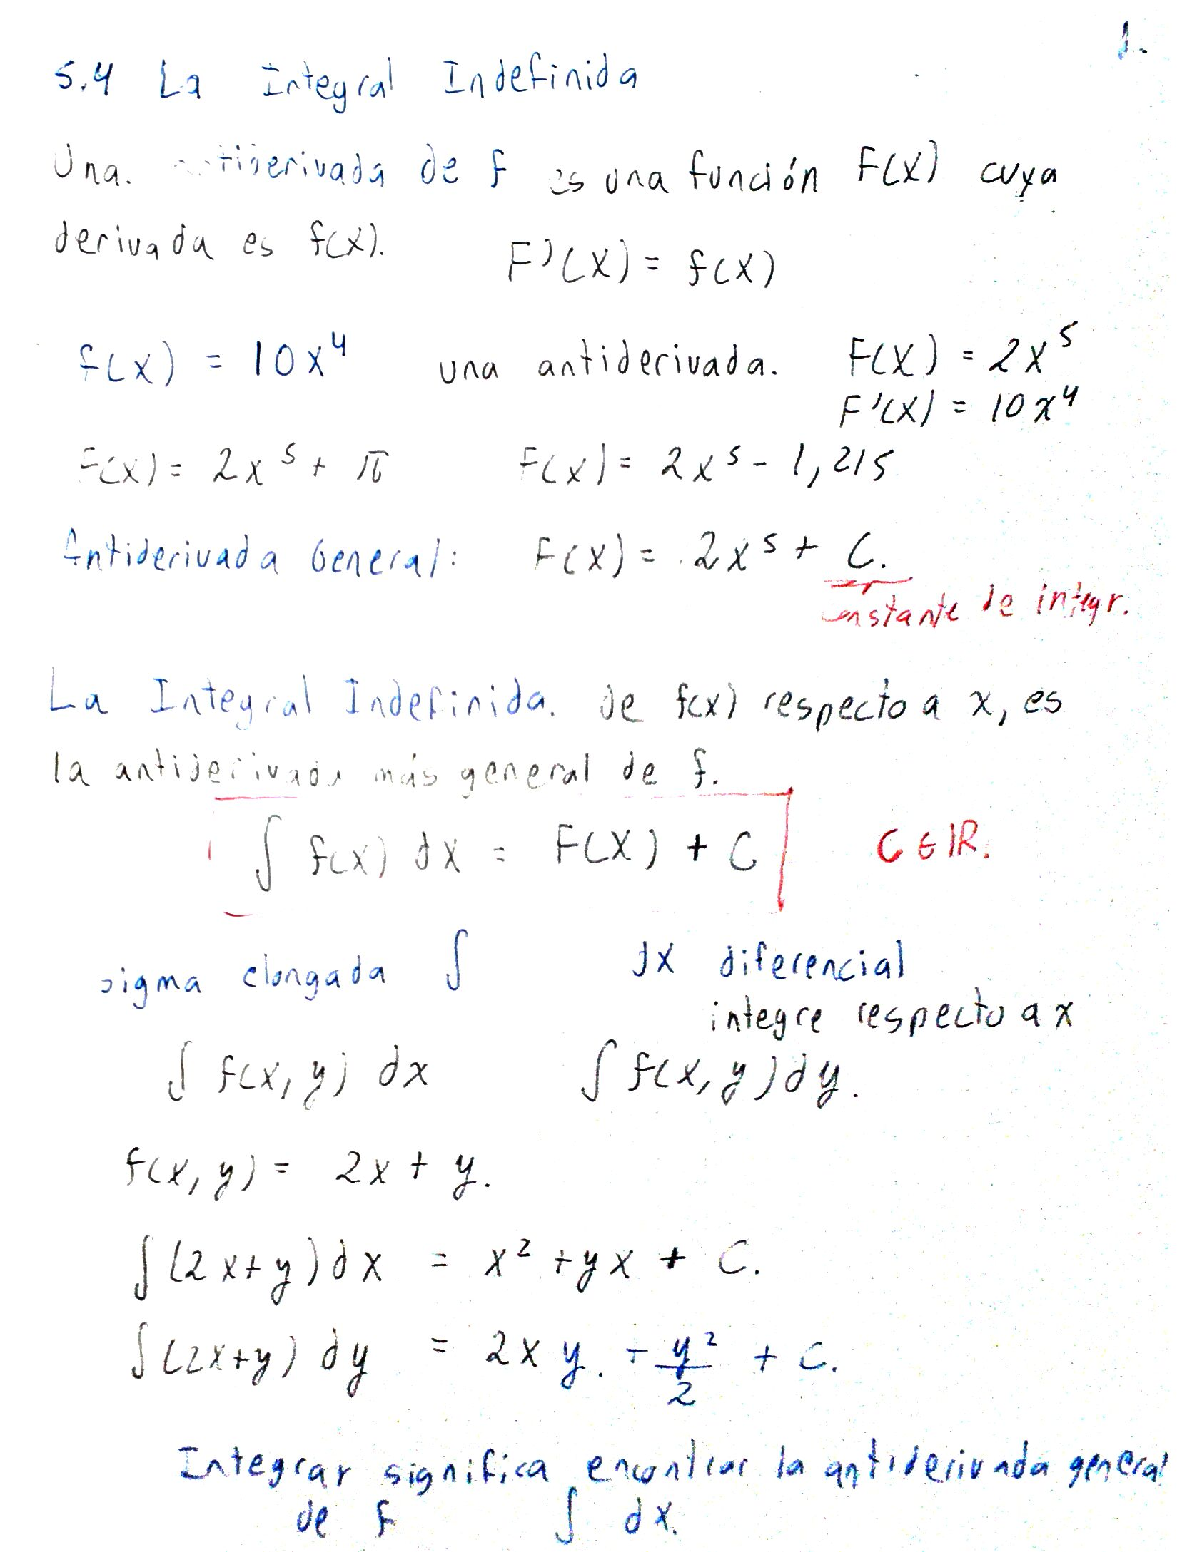
\includepdf[pages=-,pagecommand={\thispagestyle{plain}}]{pdf/RB_2019-07-23_15_22_15.pdf}
%%%%%%%%%%%%%%%%%%%%%%%%%%%%%%%%%%%%%%%%%%%%%%%%%%%%%%%%%%%%%%%%%%%%%%%%%%%%%%%%%%%%%%%%%%%%%%%%

\chapter{5.4 Áreas y propiedades de la integral definida} 
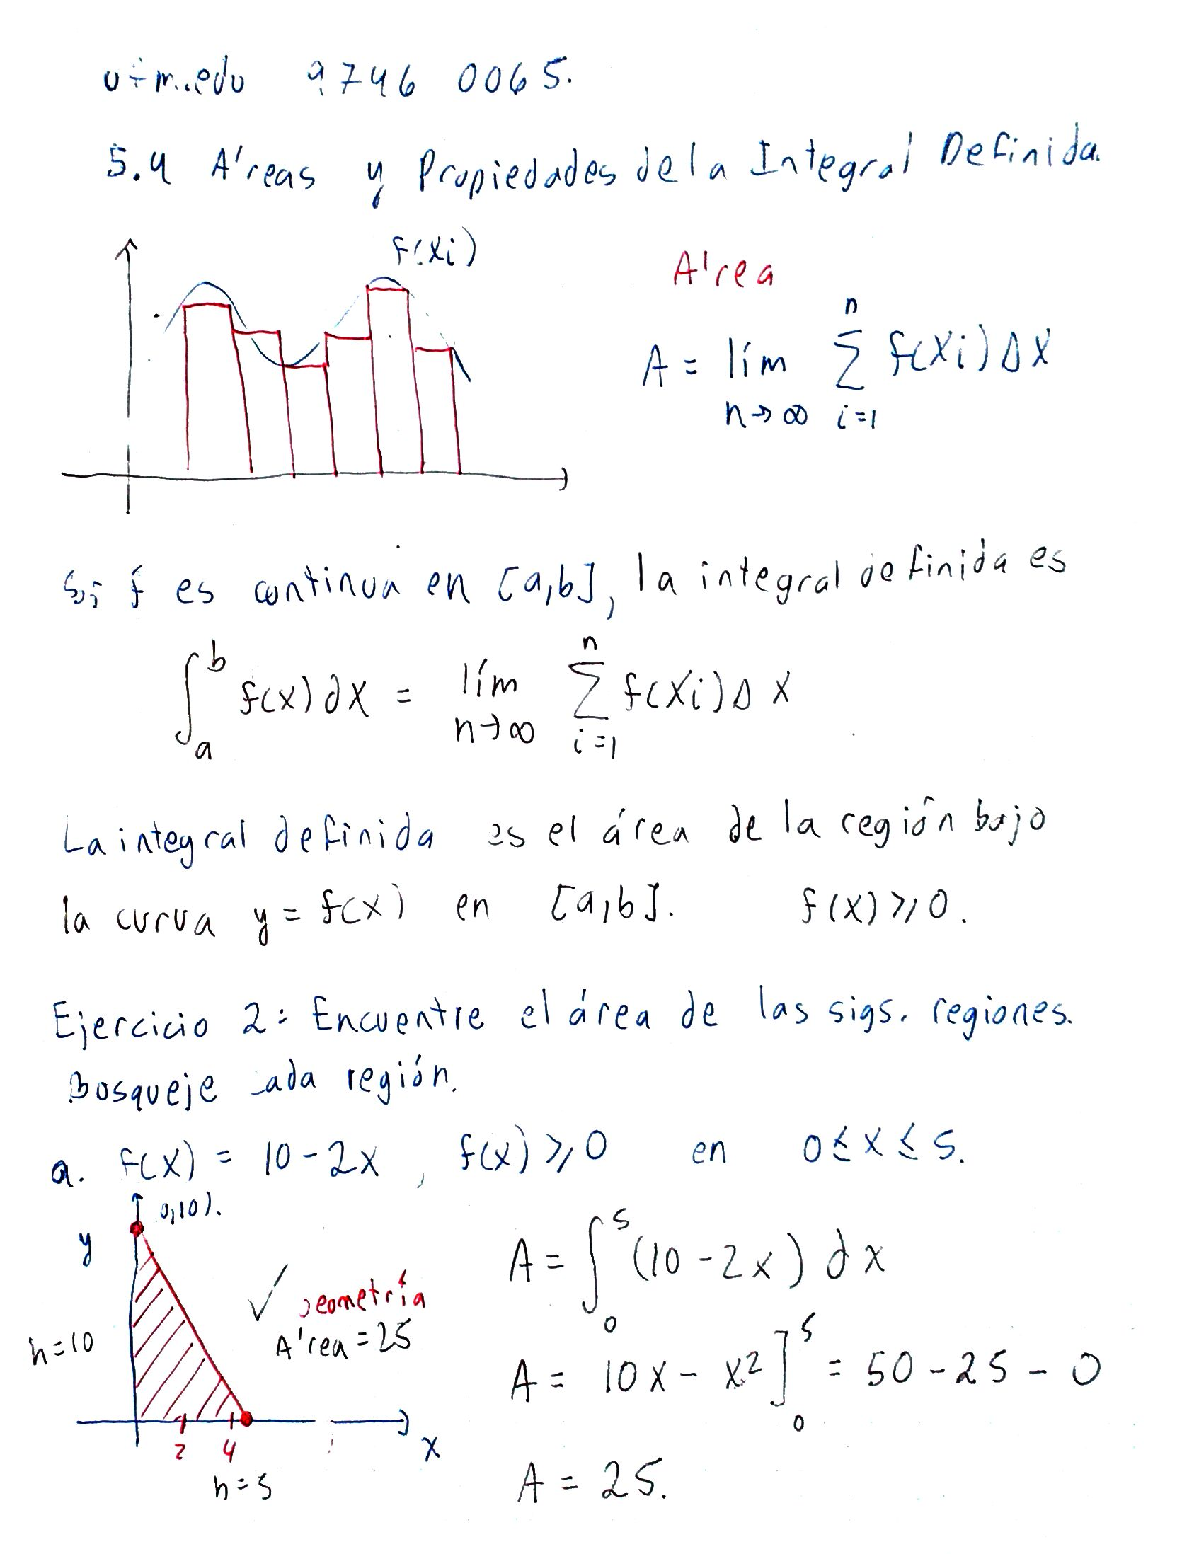
\includepdf[pages=-,pagecommand={\thispagestyle{plain}}]{pdf/RB_2019-07-25_18_26_27.pdf}
%%%%%%%%%%%%%%%%%%%%%%%%%%%%%%%%%%%%%%%%%%%%%%%%%%%%%%%%%%%%%%%%%%%%%%%%%%%%%%%%%%%%%%%%%%%%%%%%

\chapter{Desplazamiento y distancias con integrales} 
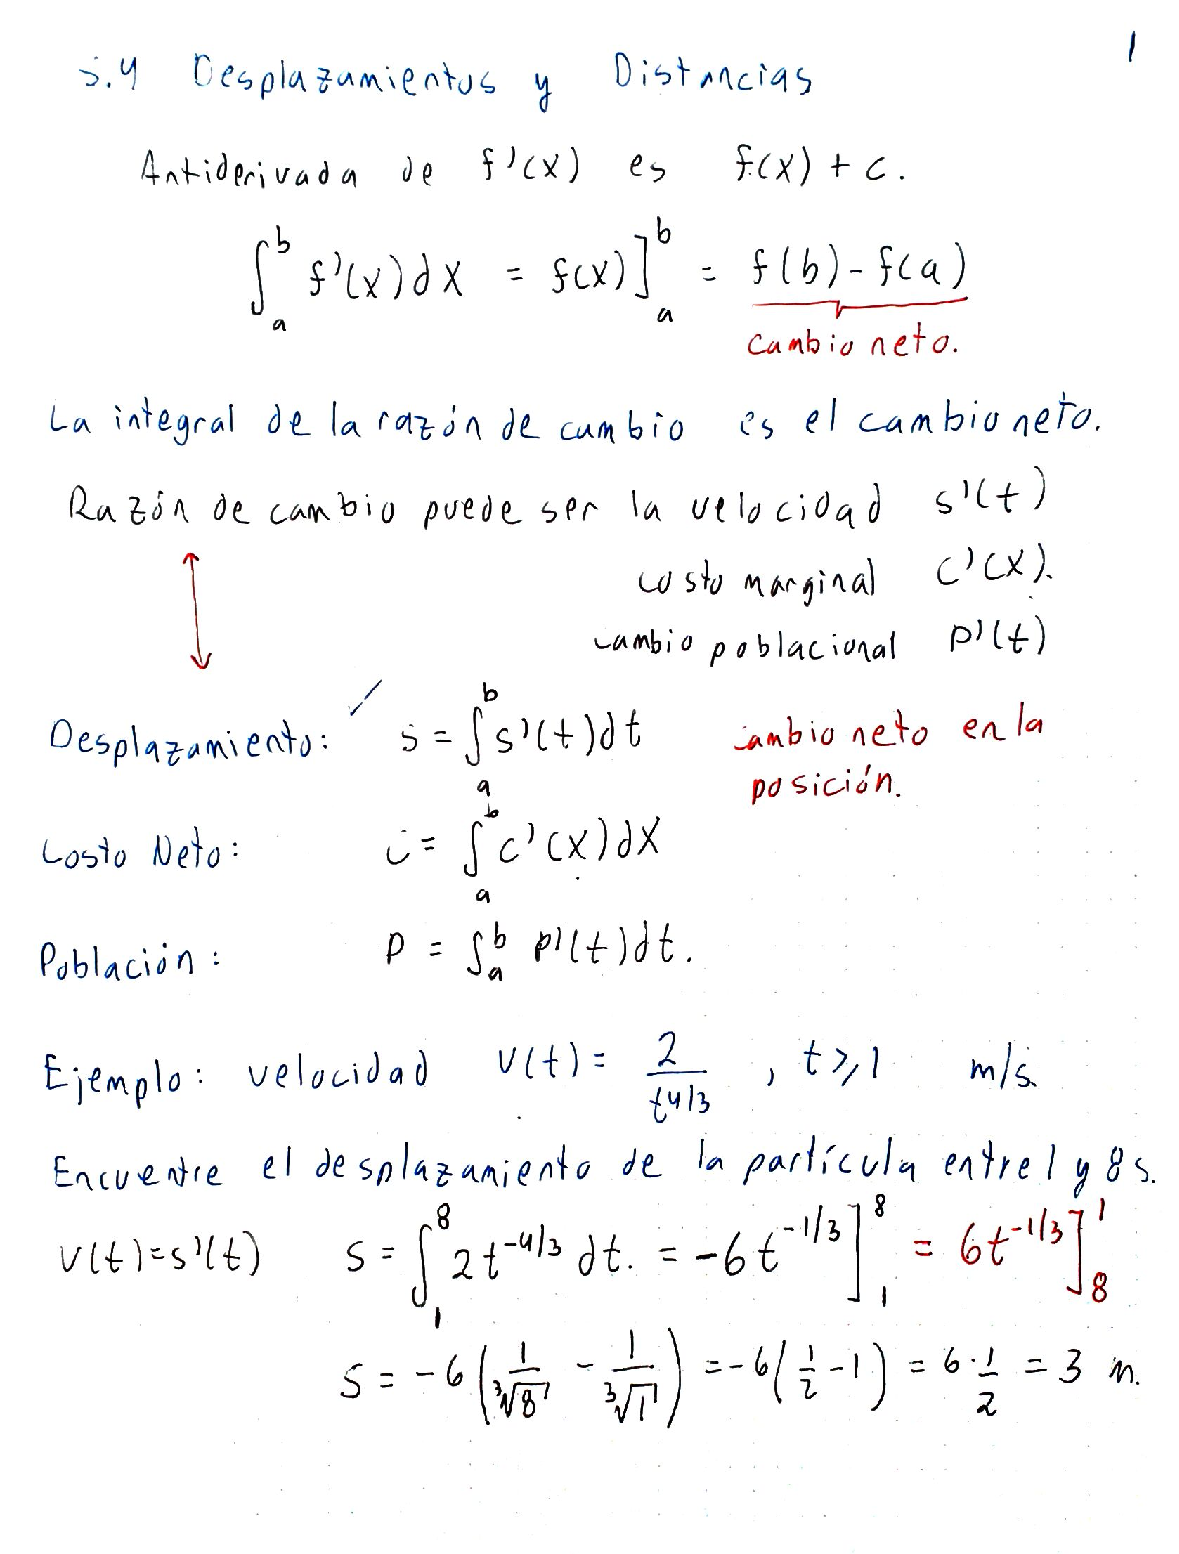
\includepdf[pages=-,pagecommand={\thispagestyle{plain}}]{pdf/RB_2019-07-30_16_36_38.pdf}
%%%%%%%%%%%%%%%%%%%%%%%%%%%%%%%%%%%%%%%%%%%%%%%%%%%%%%%%%%%%%%%%%%%%%%%%%%%%%%%%%%%%%%%%%%%%%%%%

\chapter{Teorema fundamental del cálculo, parte I \& II, derivadas de funciones compuestas y definidas para integrales, generalizaciones de TFC} 
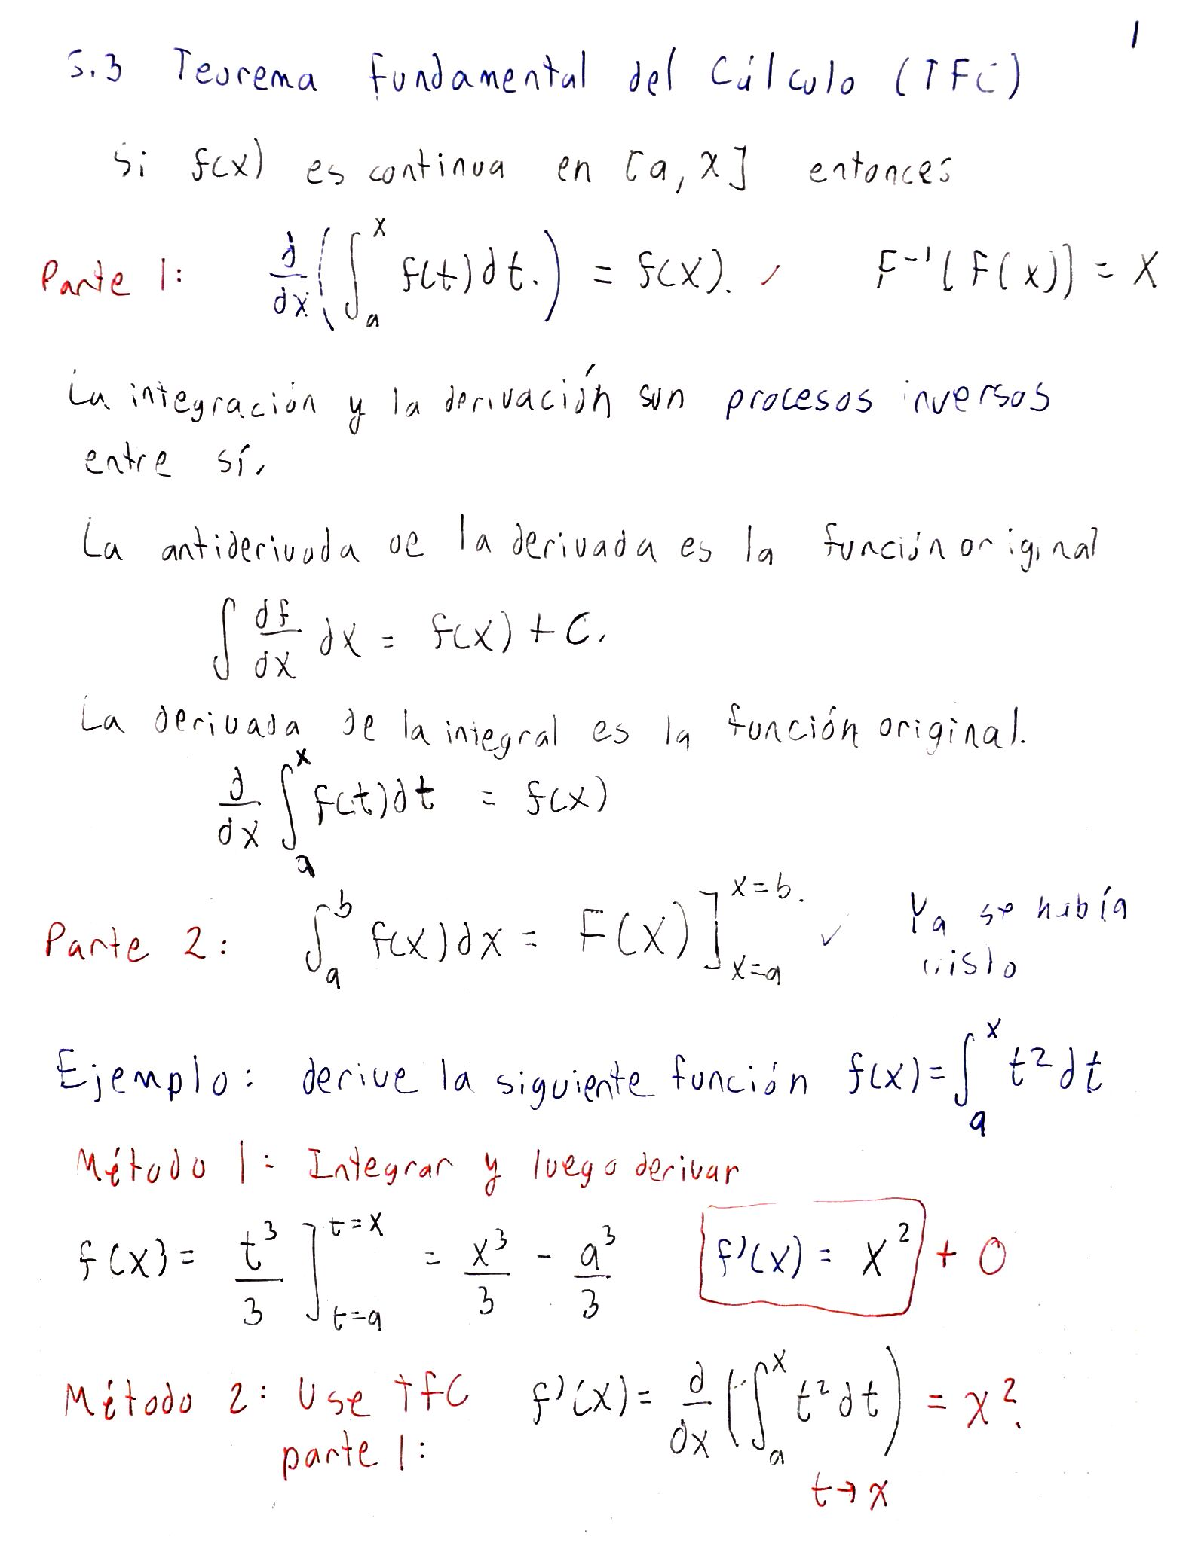
\includepdf[pages=-,pagecommand={\thispagestyle{plain}}]{pdf/RB_2019-08-01_11_35_28.pdf}
%%%%%%%%%%%%%%%%%%%%%%%%%%%%%%%%%%%%%%%%%%%%%%%%%%%%%%%%%%%%%%%%%%%%%%%%%%%%%%%%%%%%%%%%%%%%%%%%

\chapter{Técnica de integración por sustitución, para integrales definidas e indefinidas} 
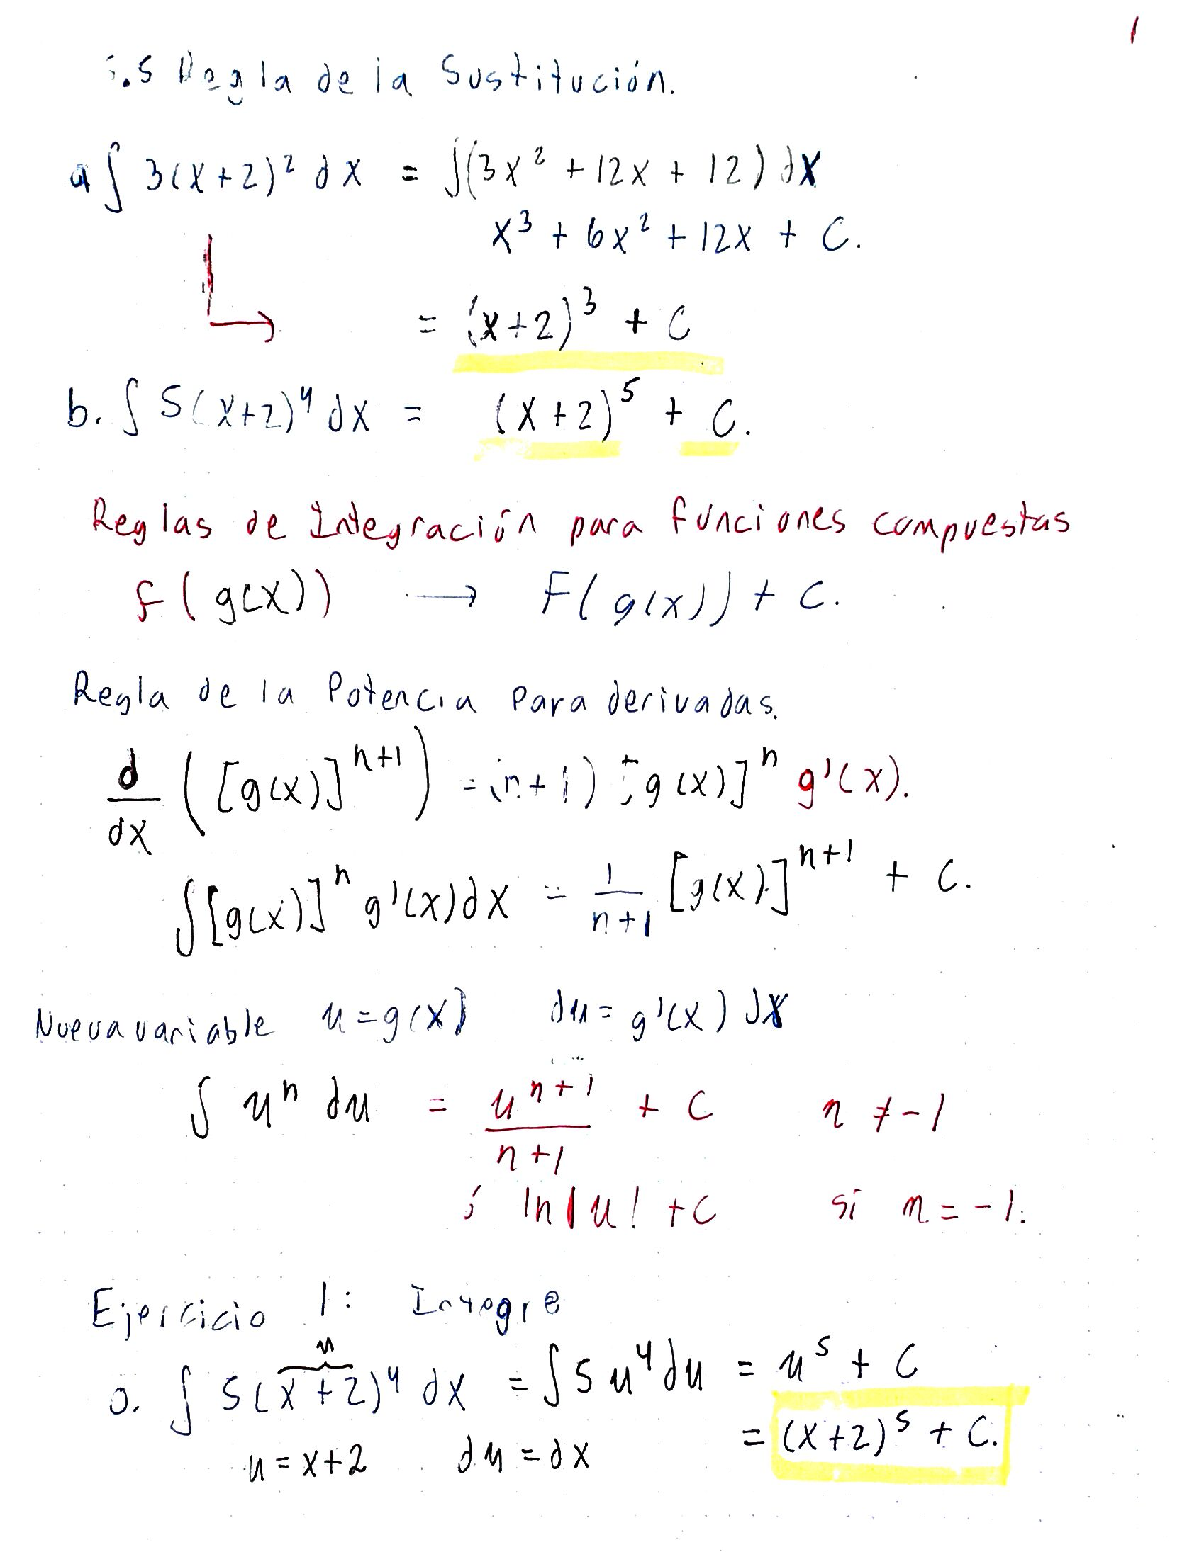
\includepdf[pages=-,pagecommand={\thispagestyle{plain}}]{pdf/RB_2019-08-06_17_50_20.pdf}
%%%%%%%%%%%%%%%%%%%%%%%%%%%%%%%%%%%%%%%%%%%%%%%%%%%%%%%%%%%%%%%%%%%%%%%%%%%%%%%%%%%%%%%%%%%%%%%%

\chapter{Técnica de integación por partes, para integrales definidas e indefinidas} 
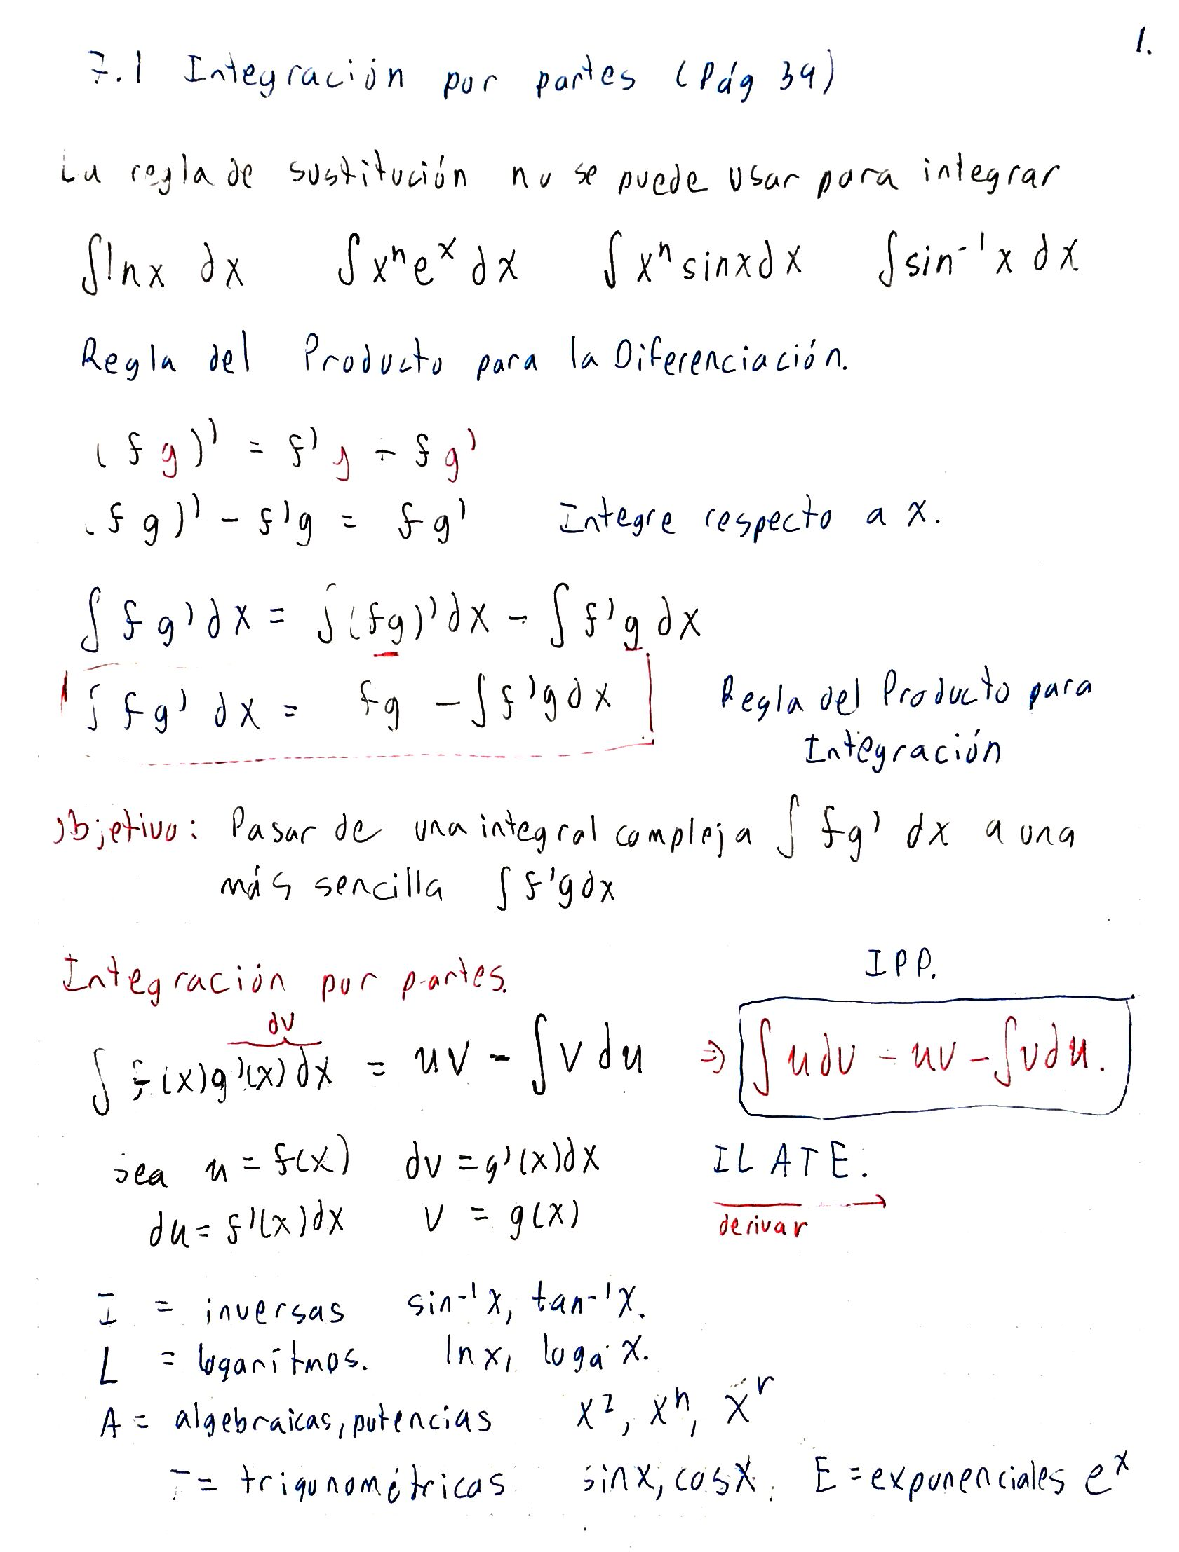
\includepdf[pages=-,pagecommand={\thispagestyle{plain}}]{pdf/RB_2019-08-08_16_16_00.pdf}
%%%%%%%%%%%%%%%%%%%%%%%%%%%%%%%%%%%%%%%%%%%%%%%%%%%%%%%%%%%%%%%%%%%%%%%%%%%%%%%%%%%%%%%%%%%%%%%%

\chapter{Integrales trigonométrias, manipulación con identidades trigonométricas de la forma \\ $1) \int \sin^n (x) \cos(x)^m dx$ \\ $2) \int \tan ^{n}(x) \sec (x)^{m} dx$ \\ $3) \int \cot^{n} (x)\sec^{m} (x) dx$} 
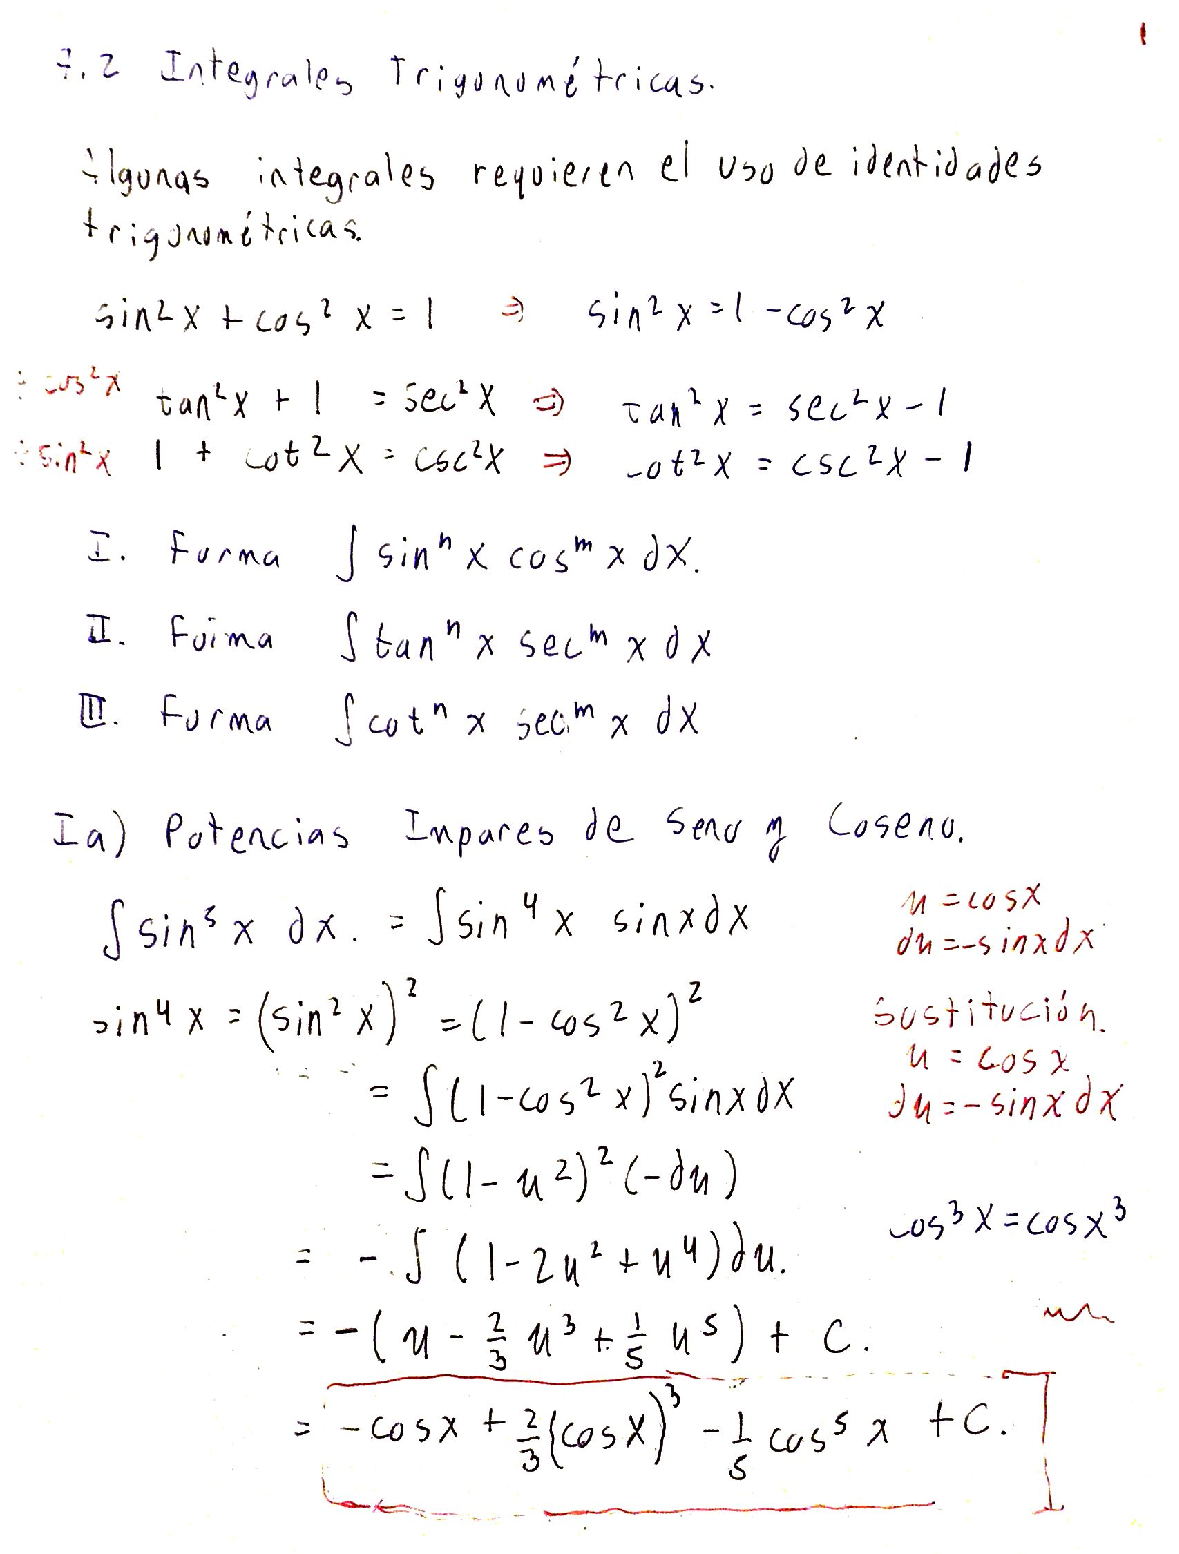
\includepdf[pages=-,pagecommand={\thispagestyle{plain}}]{pdf/RB_2019-08-13_19_21_40.pdf}
%%%%%%%%%%%%%%%%%%%%%%%%%%%%%%%%%%%%%%%%%%%%%%%%%%%%%%%%%%%%%%%%%%%%%%%%%%%%%%%%%%%%%%%%%%%%%%%%

\chapter{Integrales trigonométricas (continuación), forma \\ $1) \int \sin^n (x) \cos(x)^m dx$ \\ $2) \int sec^n(x) tan^m(x) dx$ \\ $3) \int \csc^{n}(x) \cot^{m} (x)dx$ } 
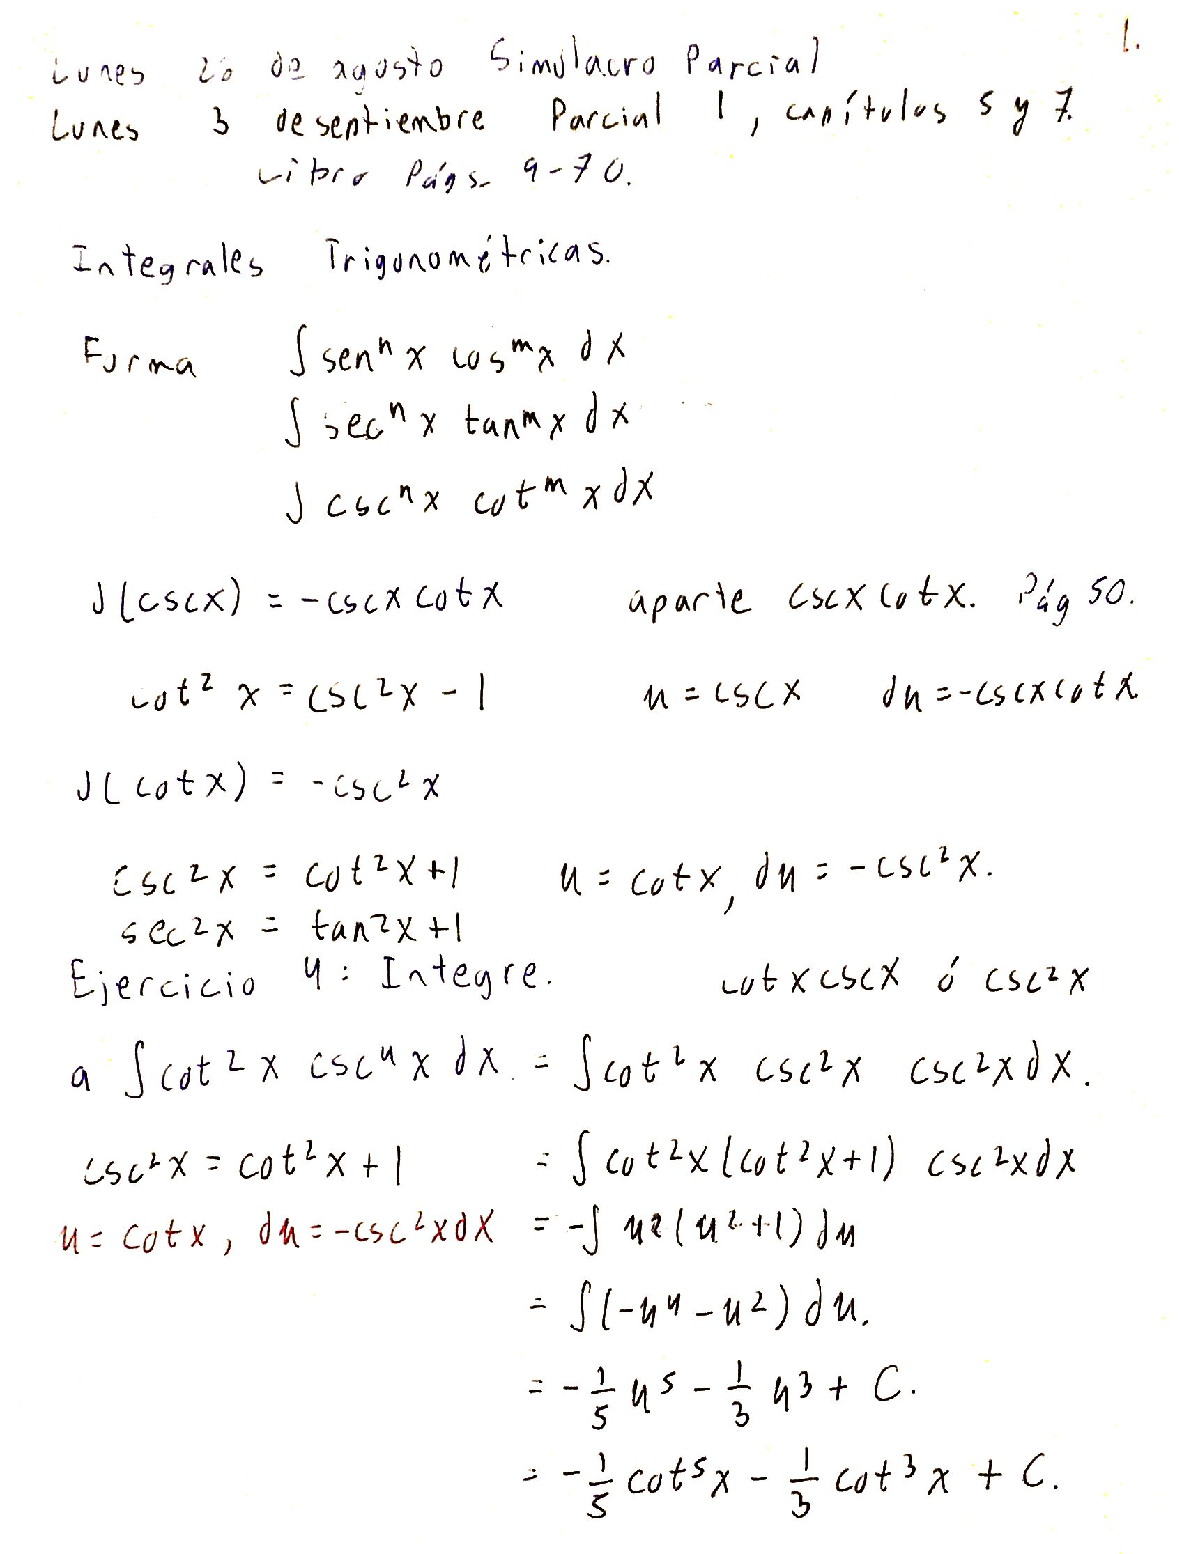
\includepdf[pages=-,pagecommand={\thispagestyle{plain}}]{pdf/RB_2019-08-20_21_49_11.pdf}
%%%%%%%%%%%%%%%%%%%%%%%%%%%%%%%%%%%%%%%%%%%%%%%%%%%%%%%%%%%%%%%%%%%%%%%%%%%%%%%%%%%%%%%%%%%%%%%%

\chapter{Sustitución trigonométrica por medio del triángulo pitagórico} 
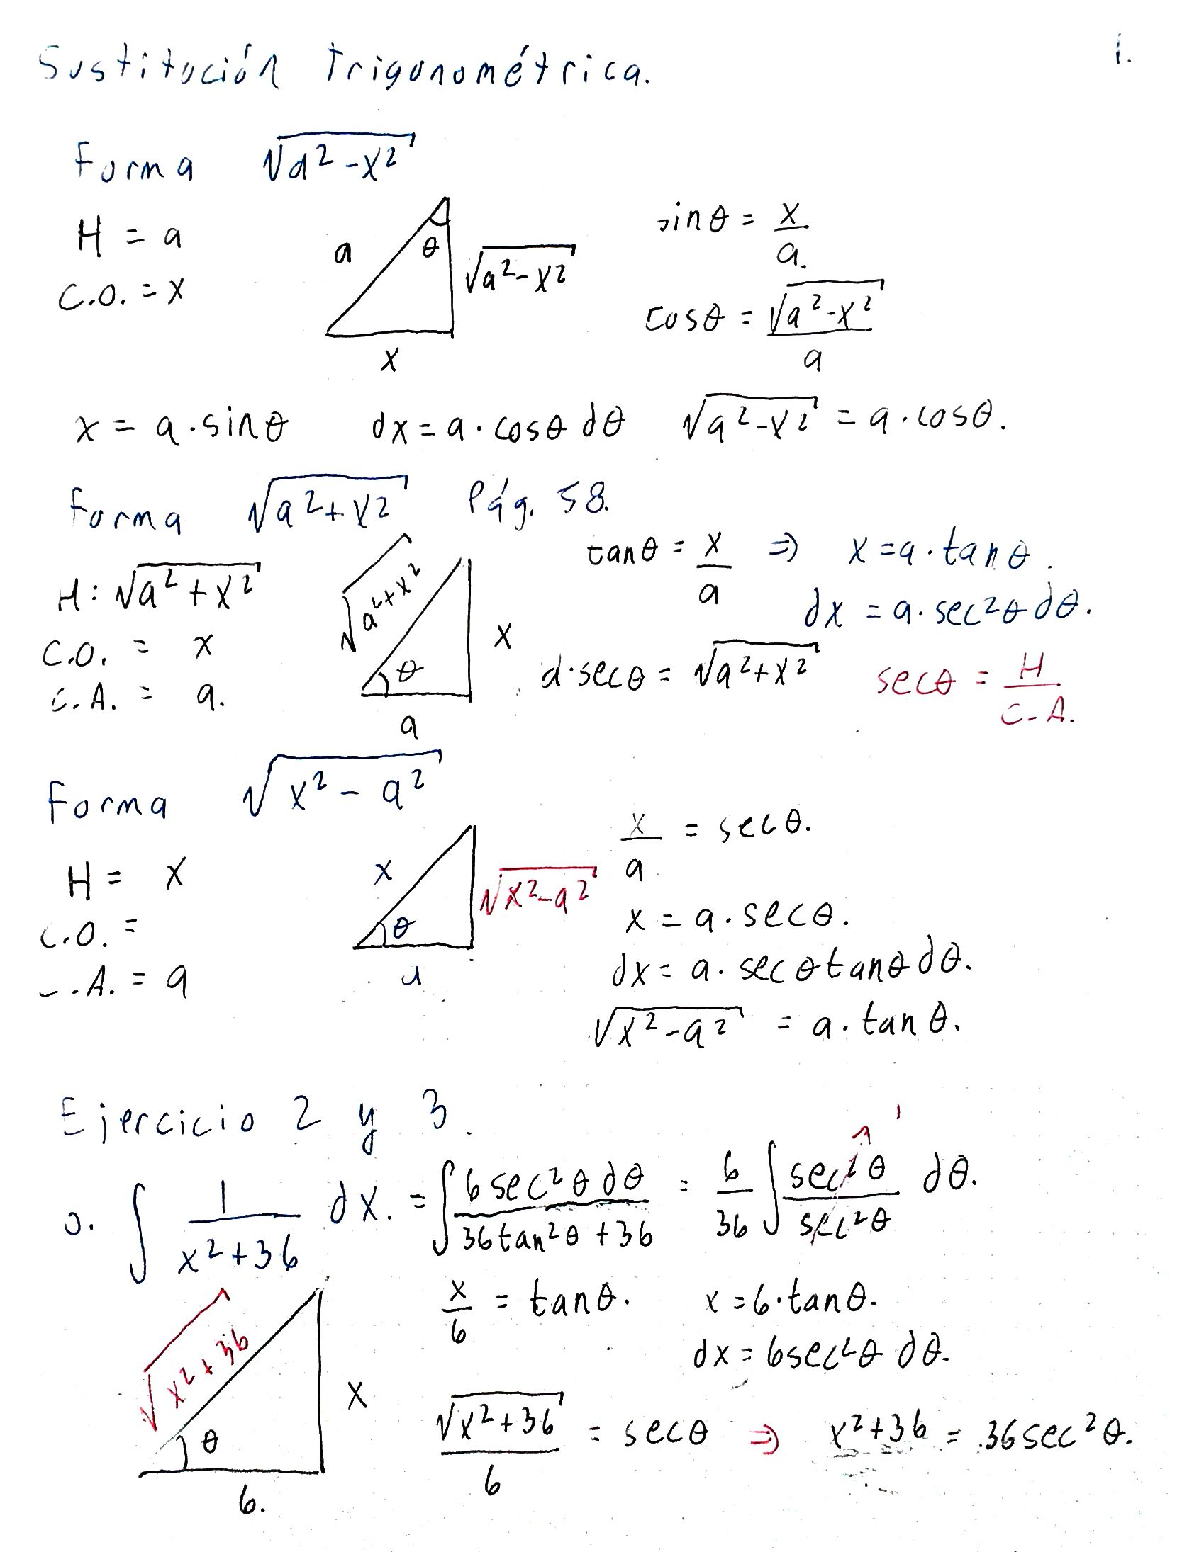
\includepdf[pages=-,pagecommand={\thispagestyle{plain}}]{pdf/RB_2019-08-23_09_43_57.pdf}
%%%%%%%%%%%%%%%%%%%%%%%%%%%%%%%%%%%%%%%%%%%%%%%%%%%%%%%%%%%%%%%%%%%%%%%%%%%%%%%%%%%%%%%%%%%%%%%%

\chapter{Más problemas de integración por sustitución trigonométrica} 
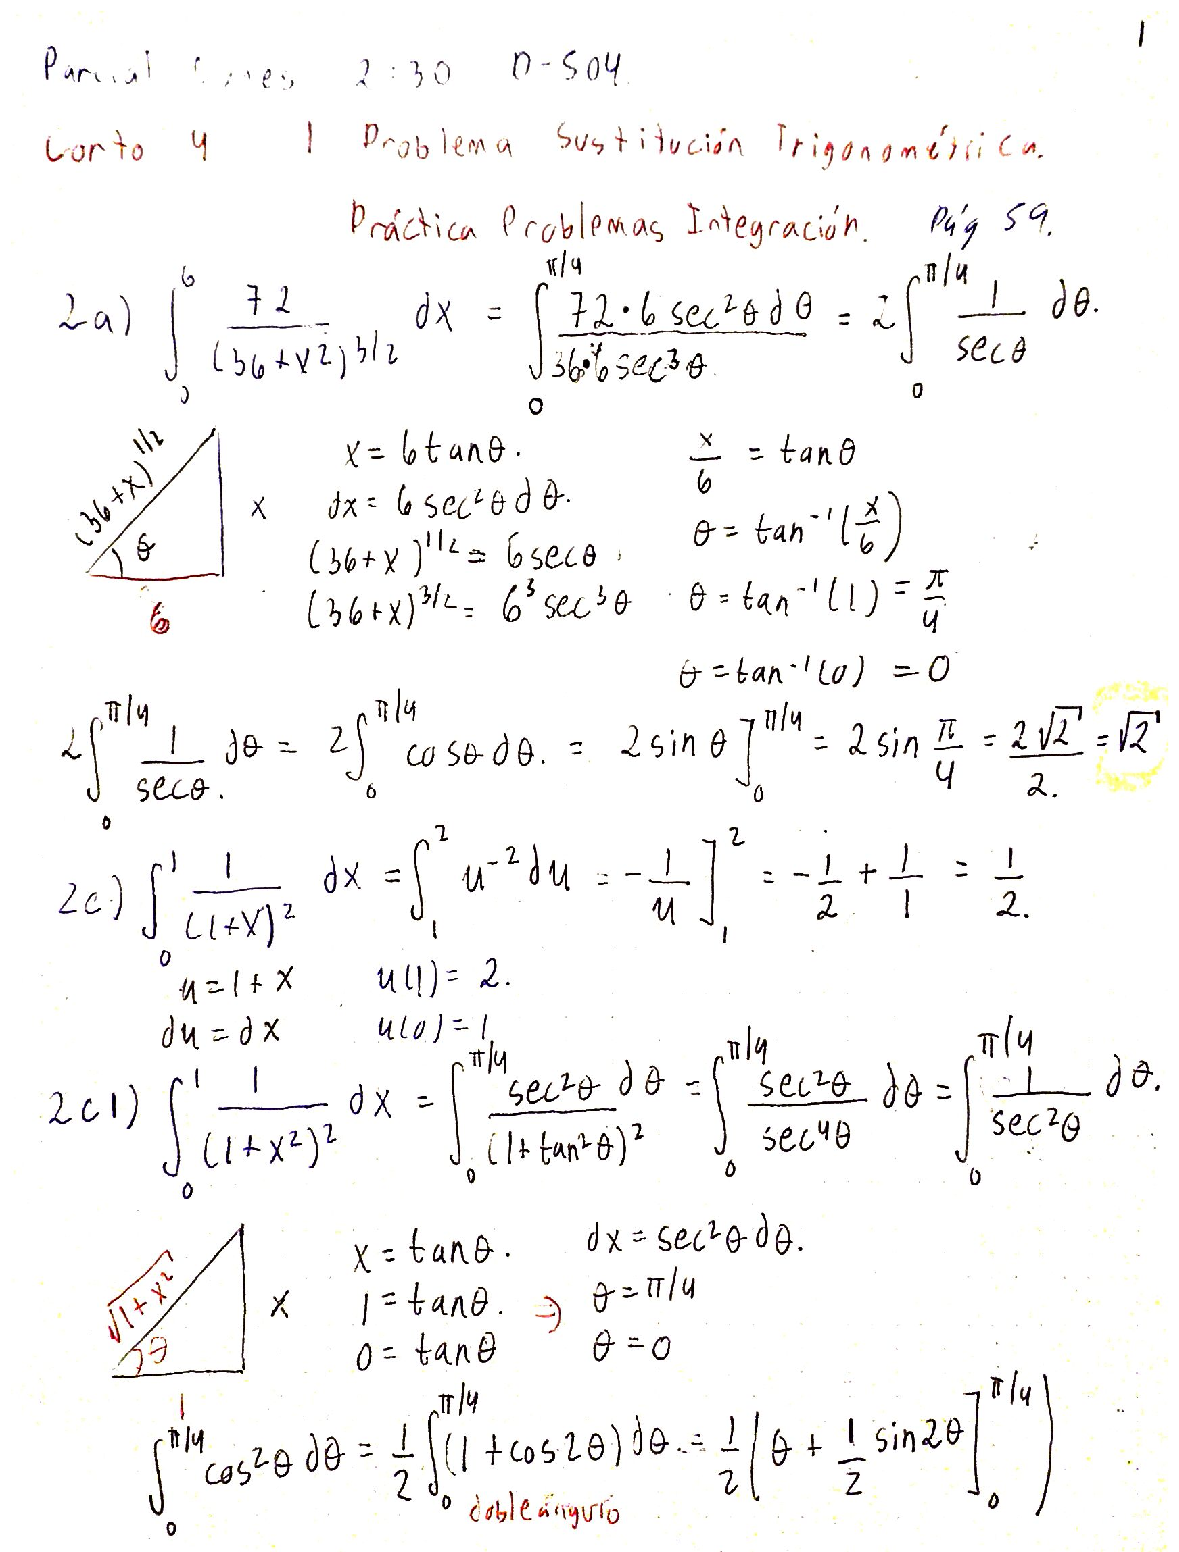
\includepdf[pages=-,pagecommand={\thispagestyle{plain}}]{pdf/RB_2019-08-27_18_00_26.pdf}
%%%%%%%%%%%%%%%%%%%%%%%%%%%%%%%%%%%%%%%%%%%%%%%%%%%%%%%%%%%%%%%%%%%%%%%%%%%%%%%%%%%%%%%%%%%%%%%%

% \chapter{ } 
% 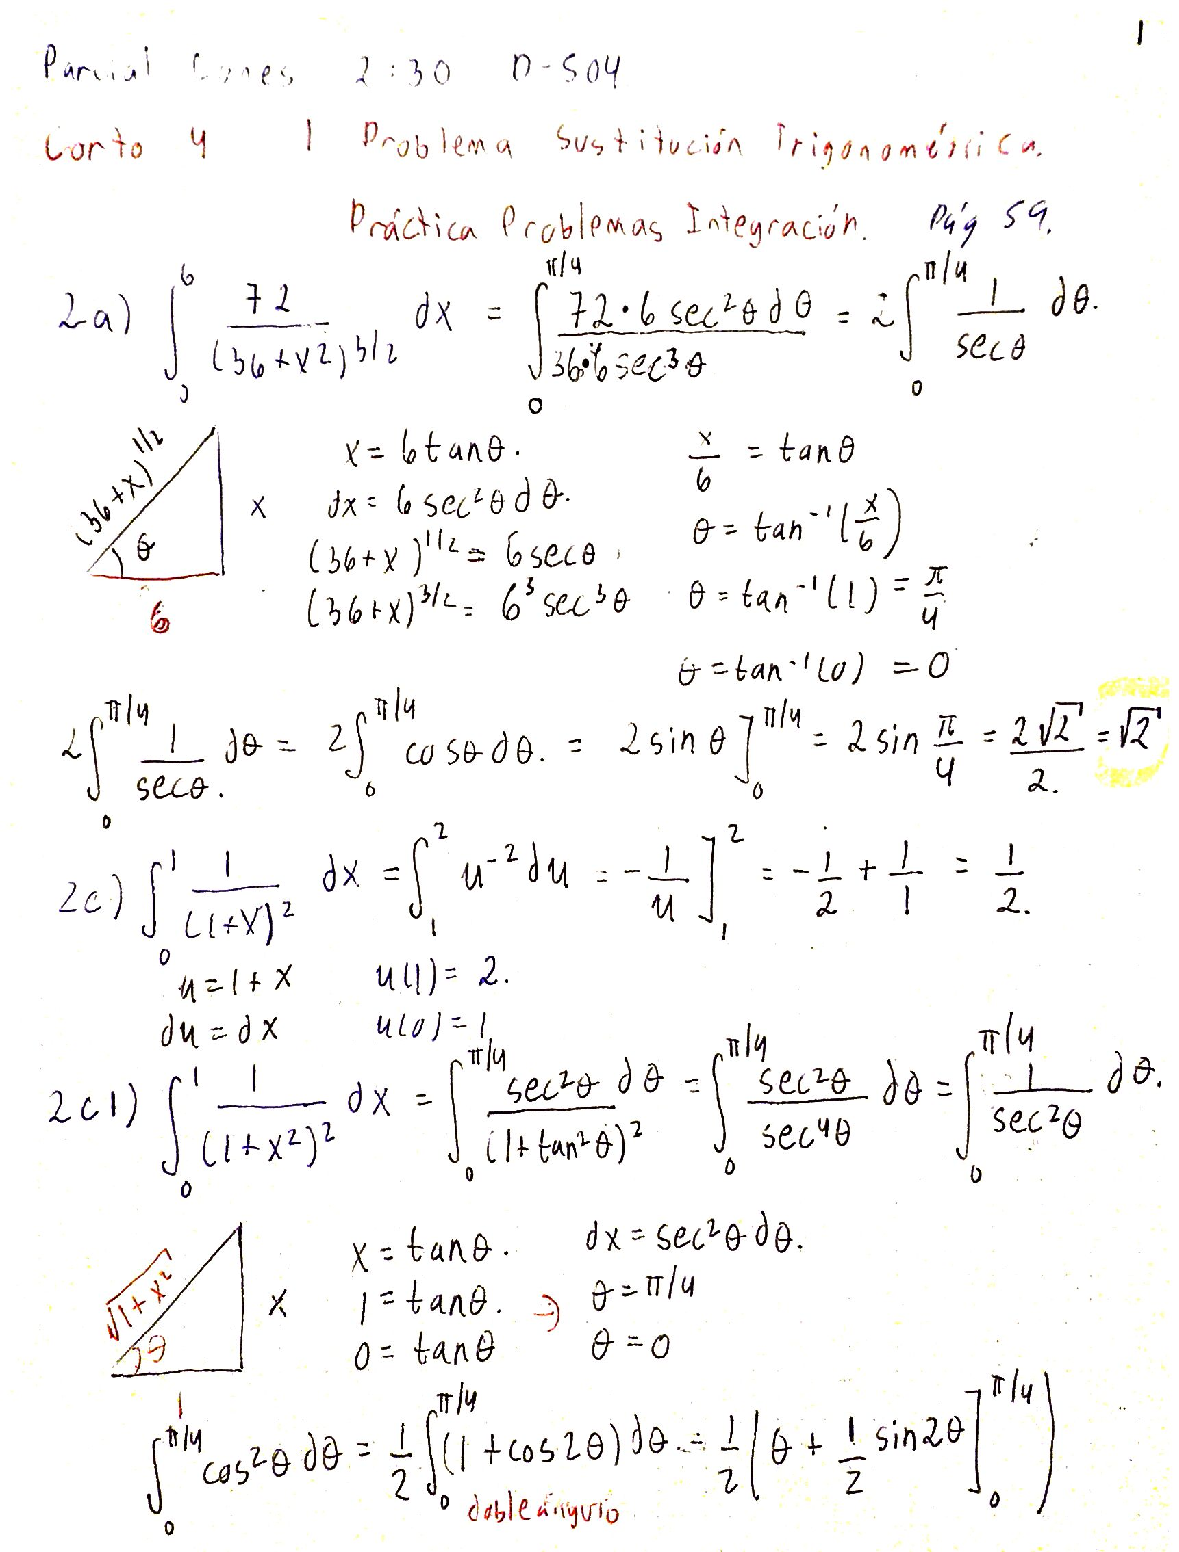
\includepdf[pages=-,pagecommand={\thispagestyle{plain}}]{pdf/RB_2019-08-27_18_04_49.pdf}
%%%%%%%%%%%%%%%%%%%%%%%%%%%%%%%%%%%%%%%%%%%%%%%%%%%%%%%%%%%%%%%%%%%%%%%%%%%%%%%%%%%%%%%%%%%%%%%%

\chapter{Simulacro de parcial \# 1} 
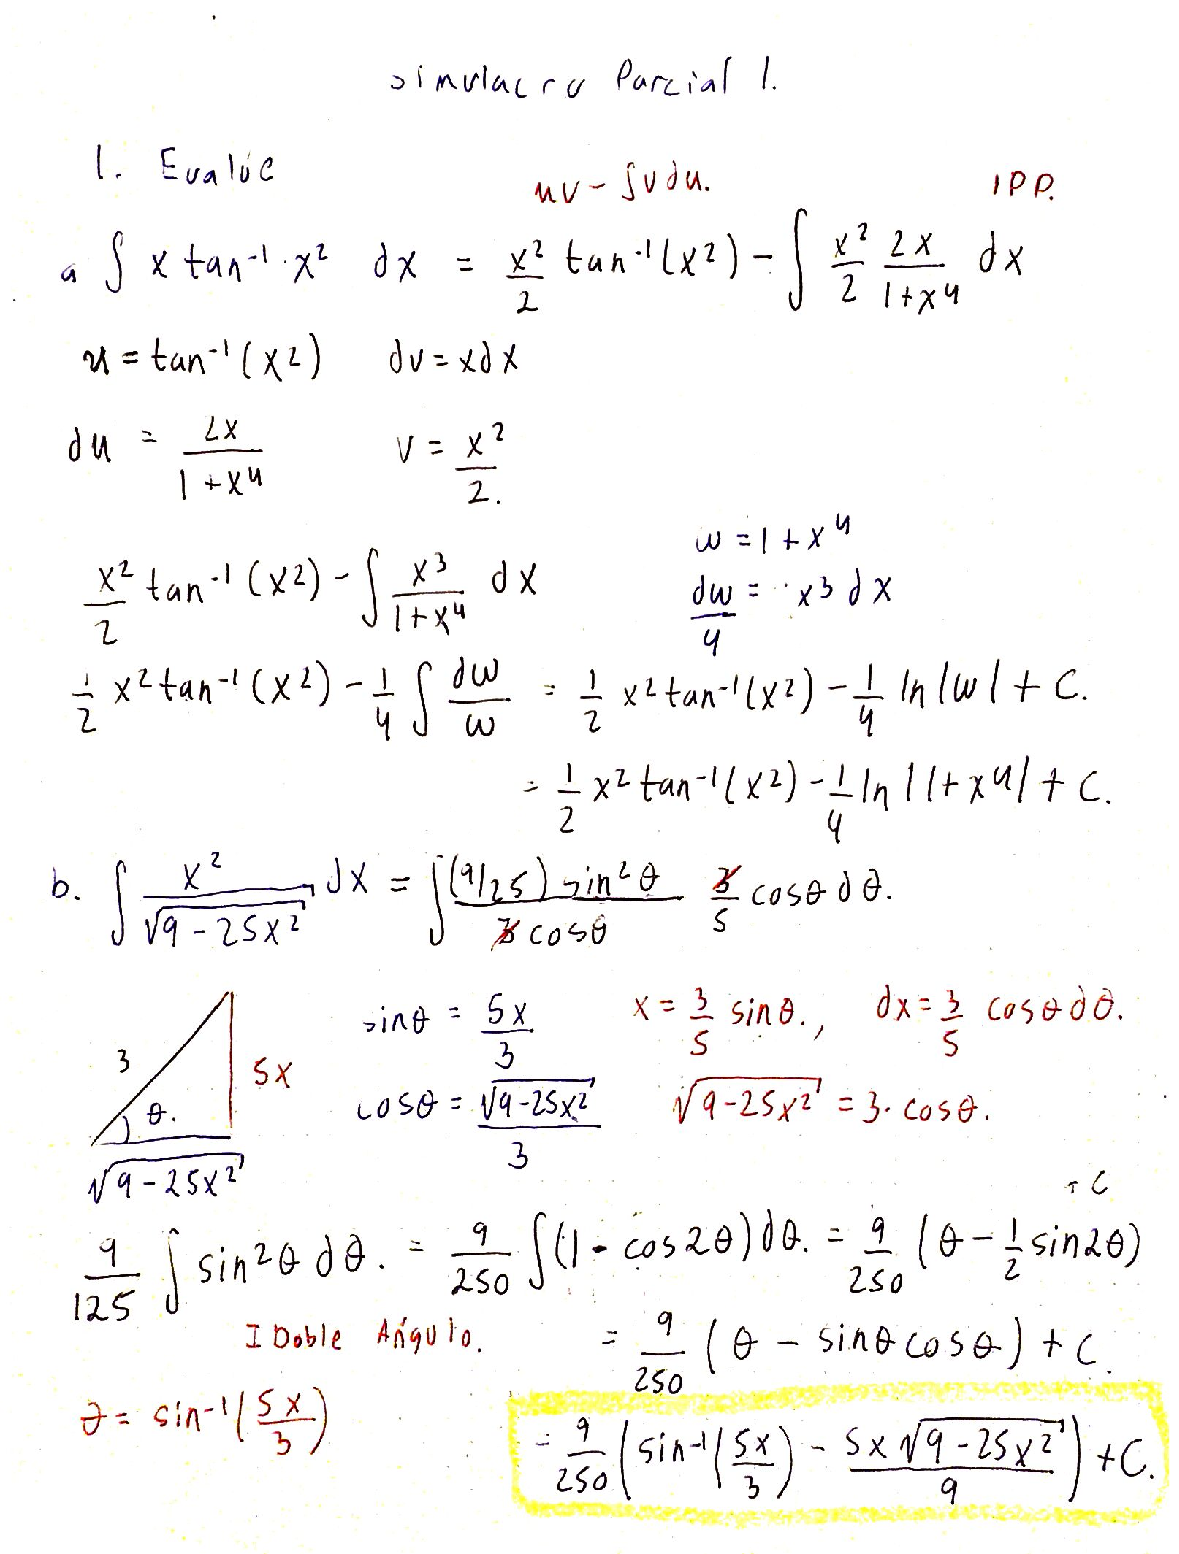
\includepdf[pages=-,pagecommand={\thispagestyle{plain}}]{pdf/RB_2019-08-29_20_18_49.pdf}
%%%%%%%%%%%%%%%%%%%%%%%%%%%%%%%%%%%%%%%%%%%%%%%%%%%%%%%%%%%%%%%%%%%%%%%%%%%%%%%%%%%%%%%%%%%%%%%%

\chapter{Integrales impropias} 
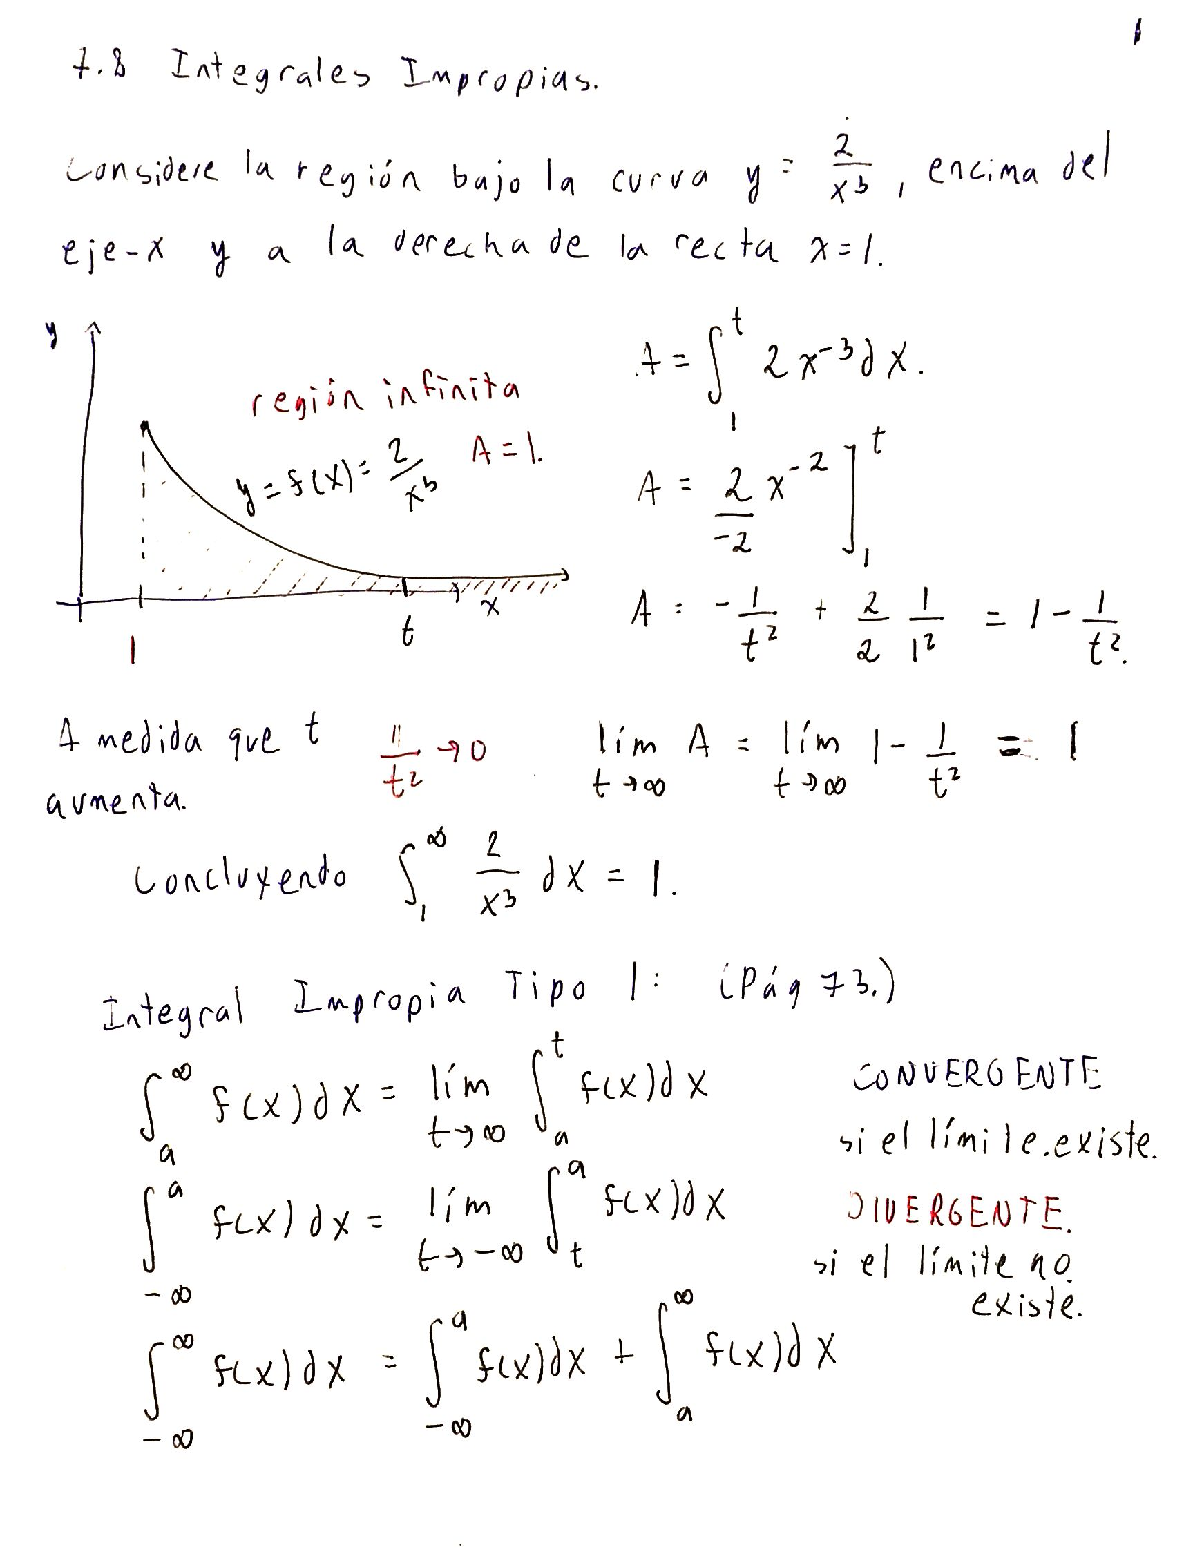
\includepdf[pages=-,pagecommand={\thispagestyle{plain}}]{pdf/RB_2019-09-03_19_54_47.pdf}
%%%%%%%%%%%%%%%%%%%%%%%%%%%%%%%%%%%%%%%%%%%%%%%%%%%%%%%%%%%%%%%%%%%%%%%%%%%%%%%%%%%%%%%%%%%%%%%%

\chapter{6.1 Área entre curvas} 
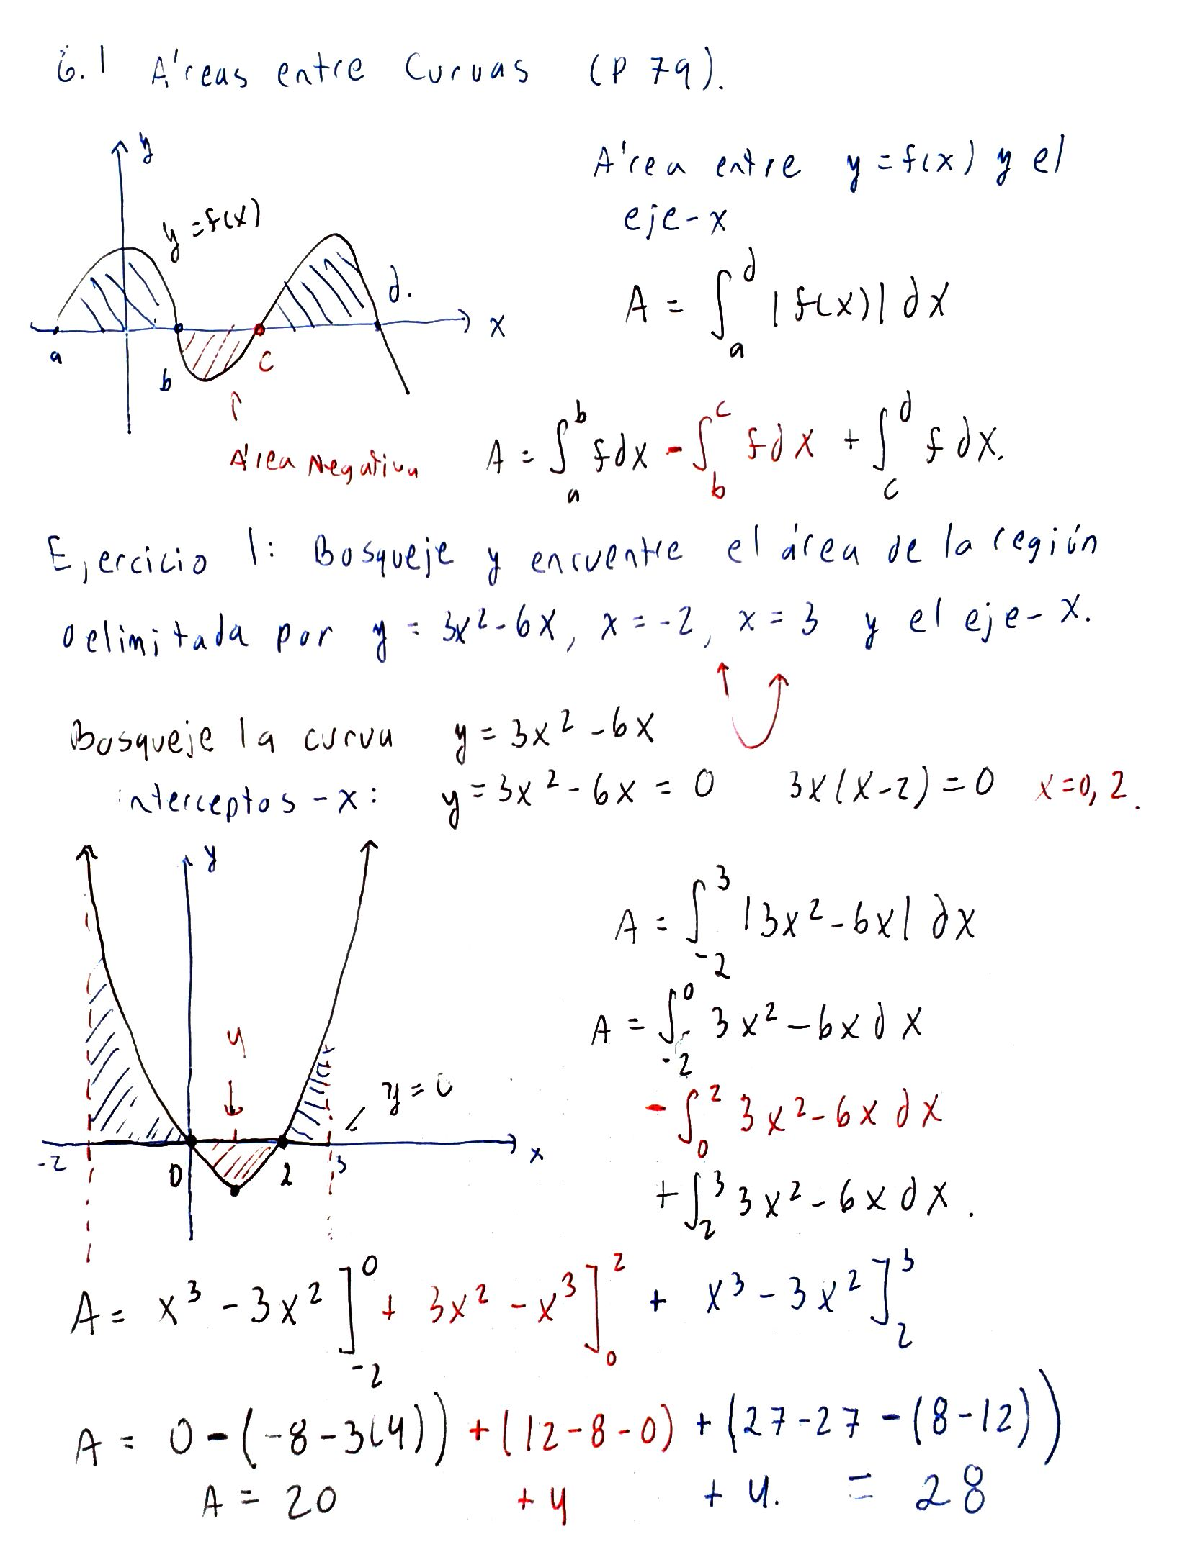
\includepdf[pages=-,pagecommand={\thispagestyle{plain}}]{pdf/RB_2019-09-06_10_55_15.pdf}
%%%%%%%%%%%%%%%%%%%%%%%%%%%%%%%%%%%%%%%%%%%%%%%%%%%%%%%%%%%%%%%%%%%%%%%%%%%%%%%%%%%%%%%%%%%%%%%%

\chapter{Área entre curvas, integración respecto al eje-y, respecto al eje-x, introducción a volúmenes de sólidos, volúmen de un cilíndro} 
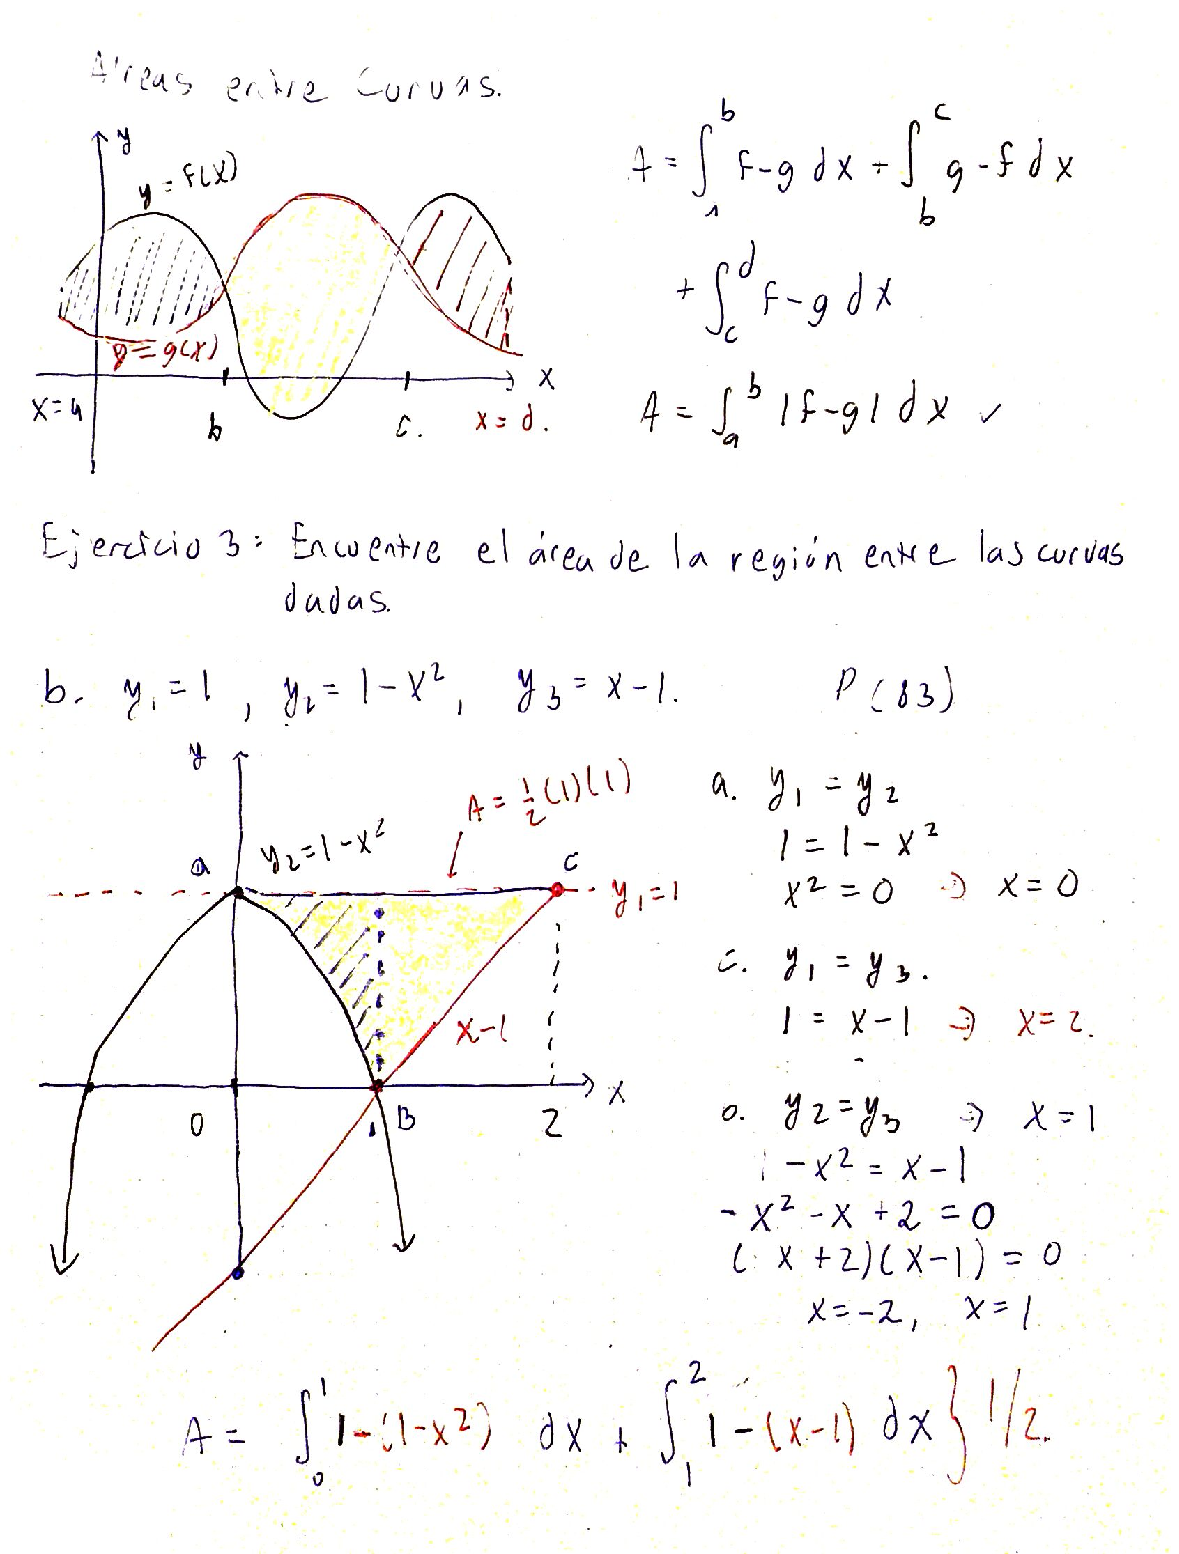
\includepdf[pages=-,pagecommand={\thispagestyle{plain}}]{pdf/RB_2019-09-10_21_23_36.pdf}
%%%%%%%%%%%%%%%%%%%%%%%%%%%%%%%%%%%%%%%%%%%%%%%%%%%%%%%%%%%%%%%%%%%%%%%%%%%%%%%%%%%%%%%%%%%%%%%%

\chapter{Volúmenes sólidos en revolución, introducción a arandelas} 
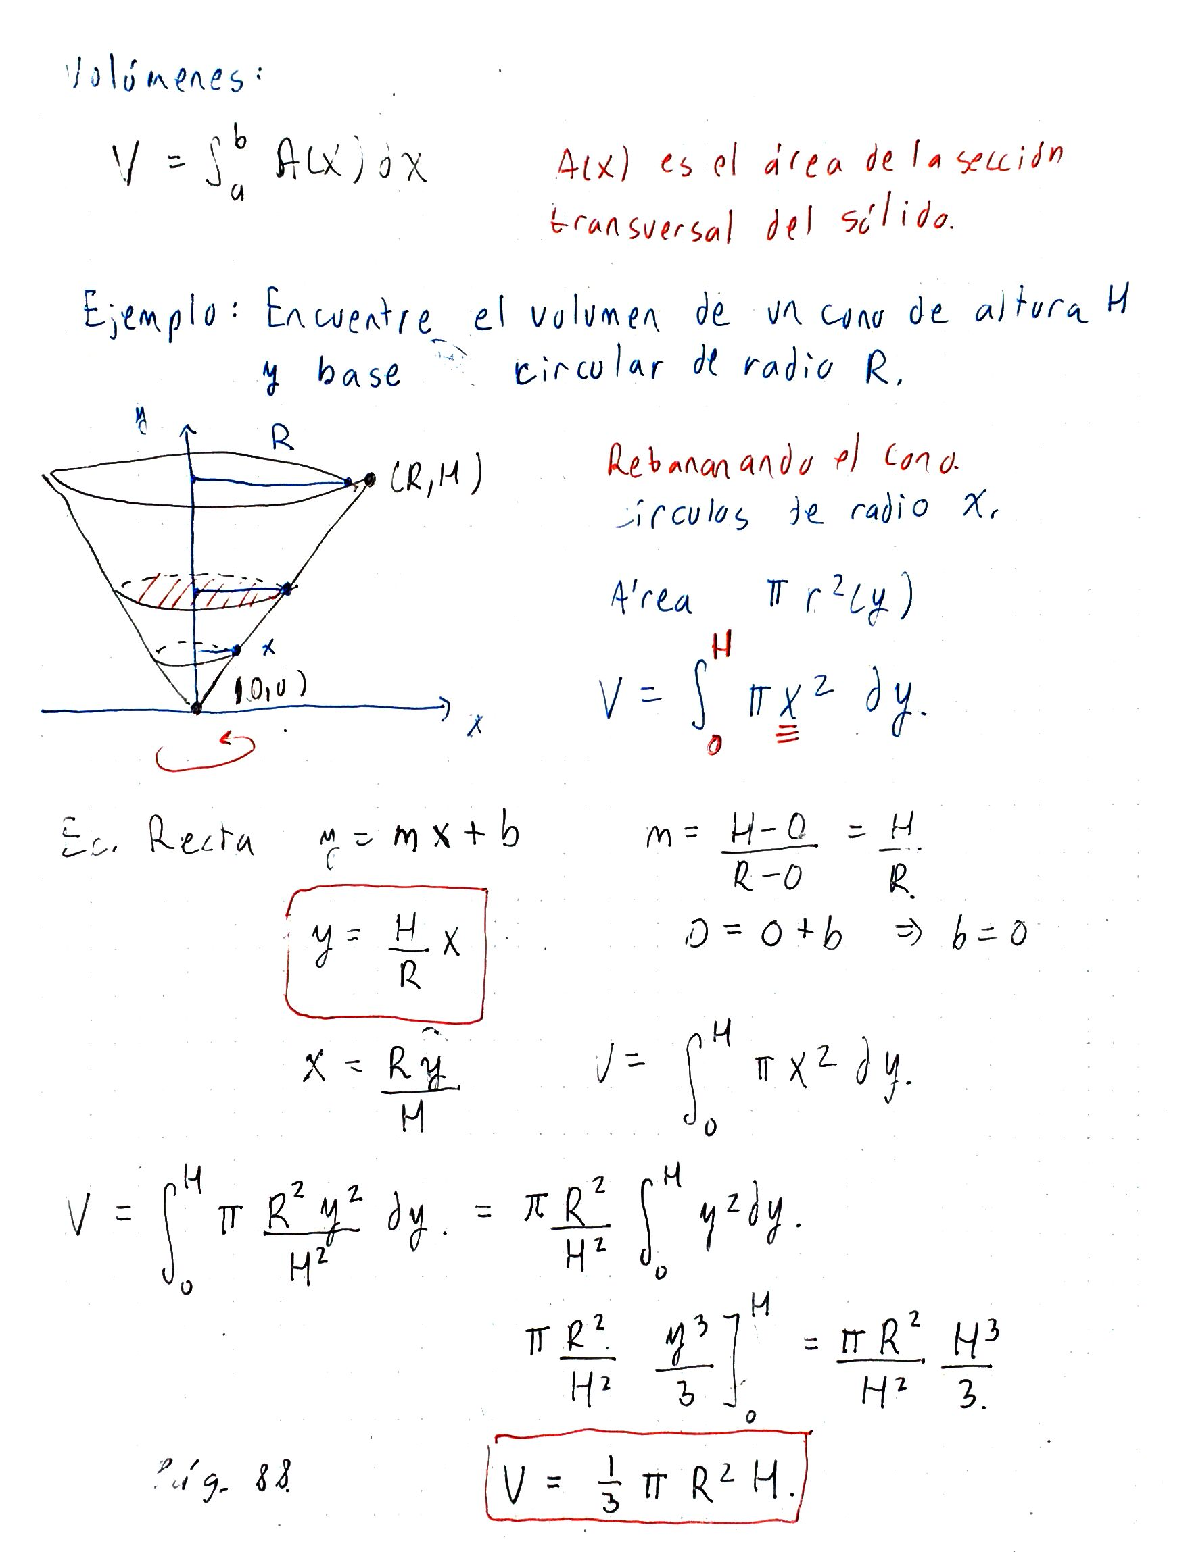
\includepdf[pages=-,pagecommand={\thispagestyle{plain}}]{pdf/RB_2019-09-12_13_52_09.pdf}
%%%%%%%%%%%%%%%%%%%%%%%%%%%%%%%%%%%%%%%%%%%%%%%%%%%%%%%%%%%%%%%%%%%%%%%%%%%%%%%%%%%%%%%%%%%%%%%%

\chapter{Volúmenes por arandelas y cascarones cilíndricos del cuadrado infinitesimal} 
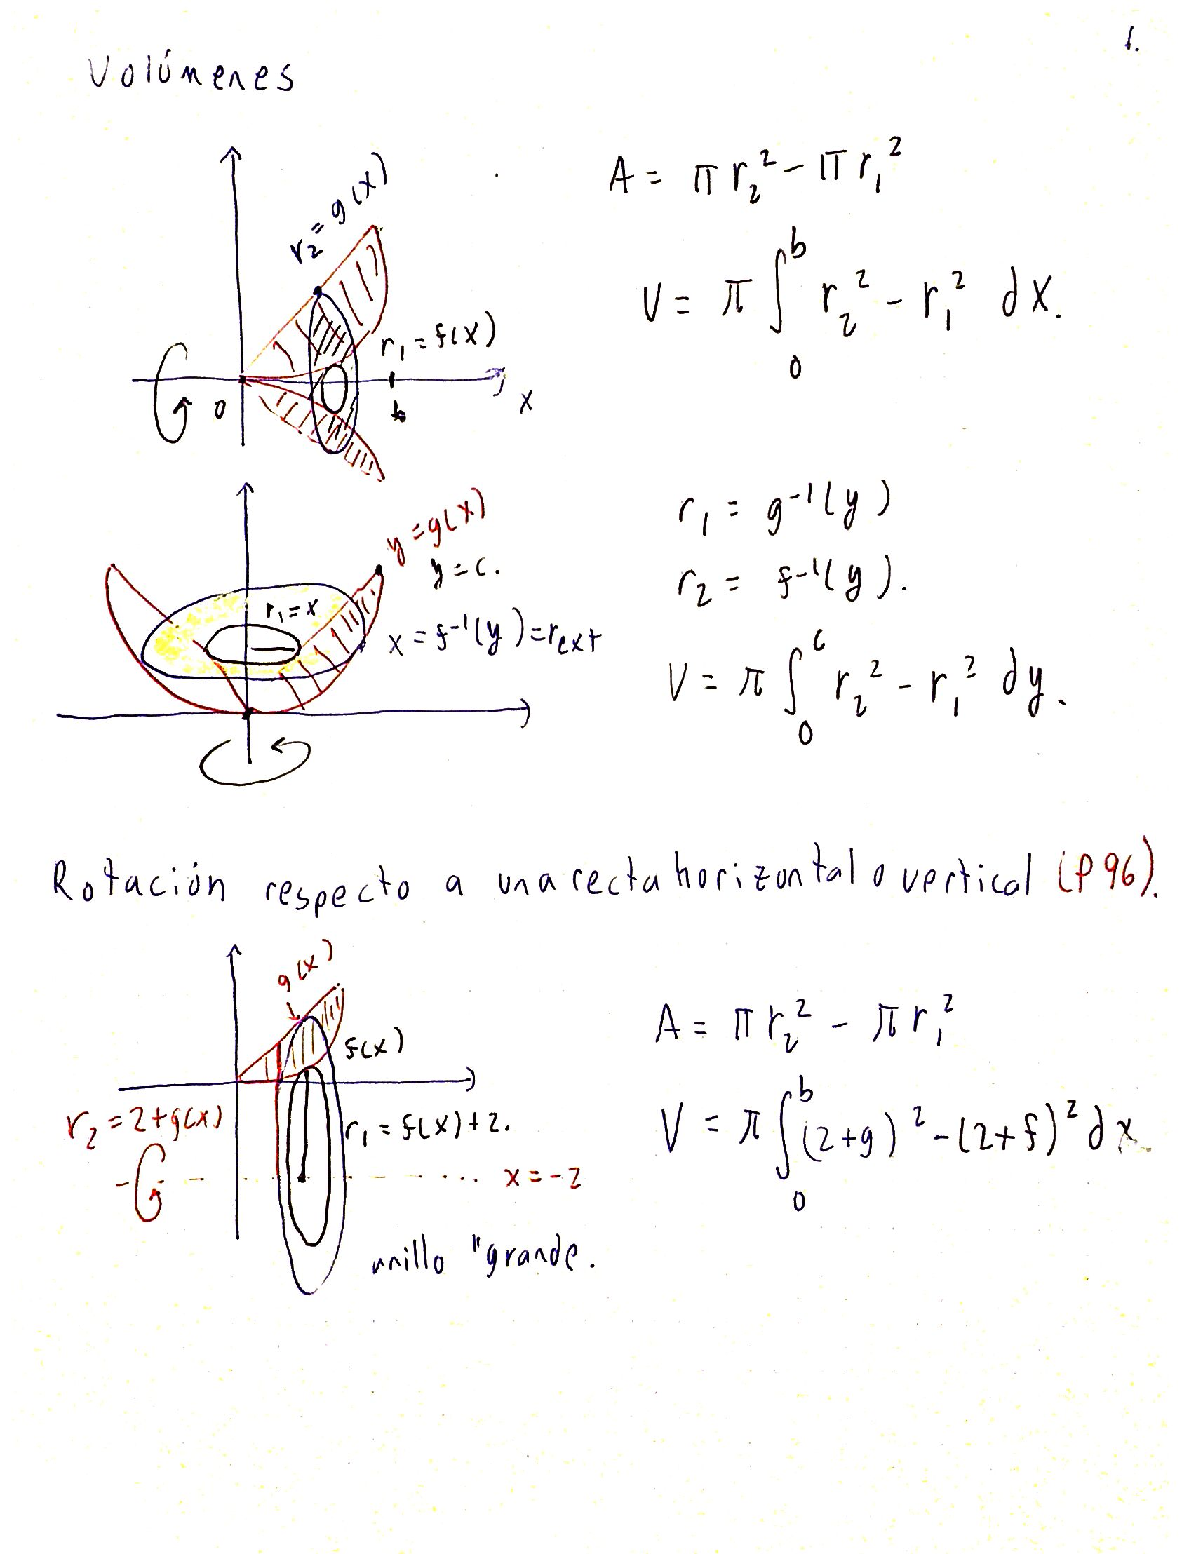
\includepdf[pages=-,pagecommand={\thispagestyle{plain}}]{pdf/RB_2019-09-17_18_59_28.pdf}
%%%%%%%%%%%%%%%%%%%%%%%%%%%%%%%%%%%%%%%%%%%%%%%%%%%%%%%%%%%%%%%%%%%%%%%%%%%%%%%%%%%%%%%%%%%%%%%%

\chapter{6.5 Valor promedio de una función } 
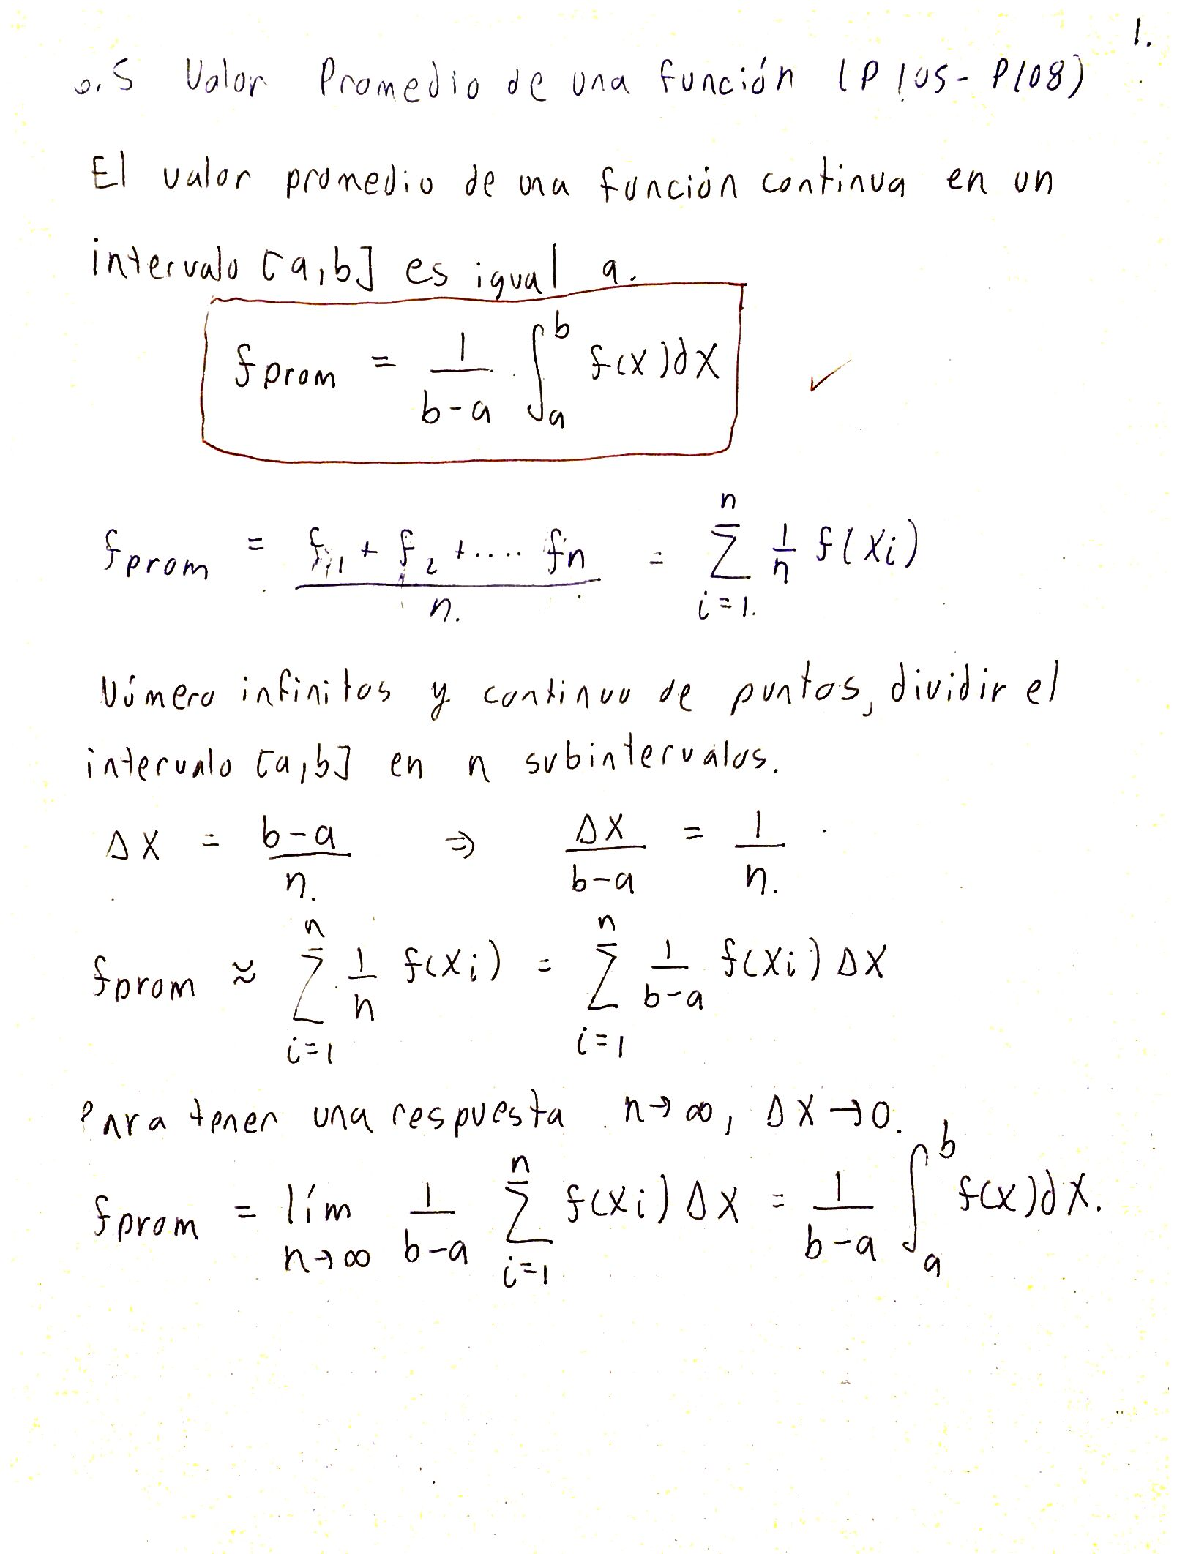
\includepdf[pages=-,pagecommand={\thispagestyle{plain}}]{pdf/RB_2019-09-19_23_09_29.pdf}
%%%%%%%%%%%%%%%%%%%%%%%%%%%%%%%%%%%%%%%%%%%%%%%%%%%%%%%%%%%%%%%%%%%%%%%%%%%%%%%%%%%%%%%%%%%%%%%%
\chapter{8.1 Longitud de arco }  
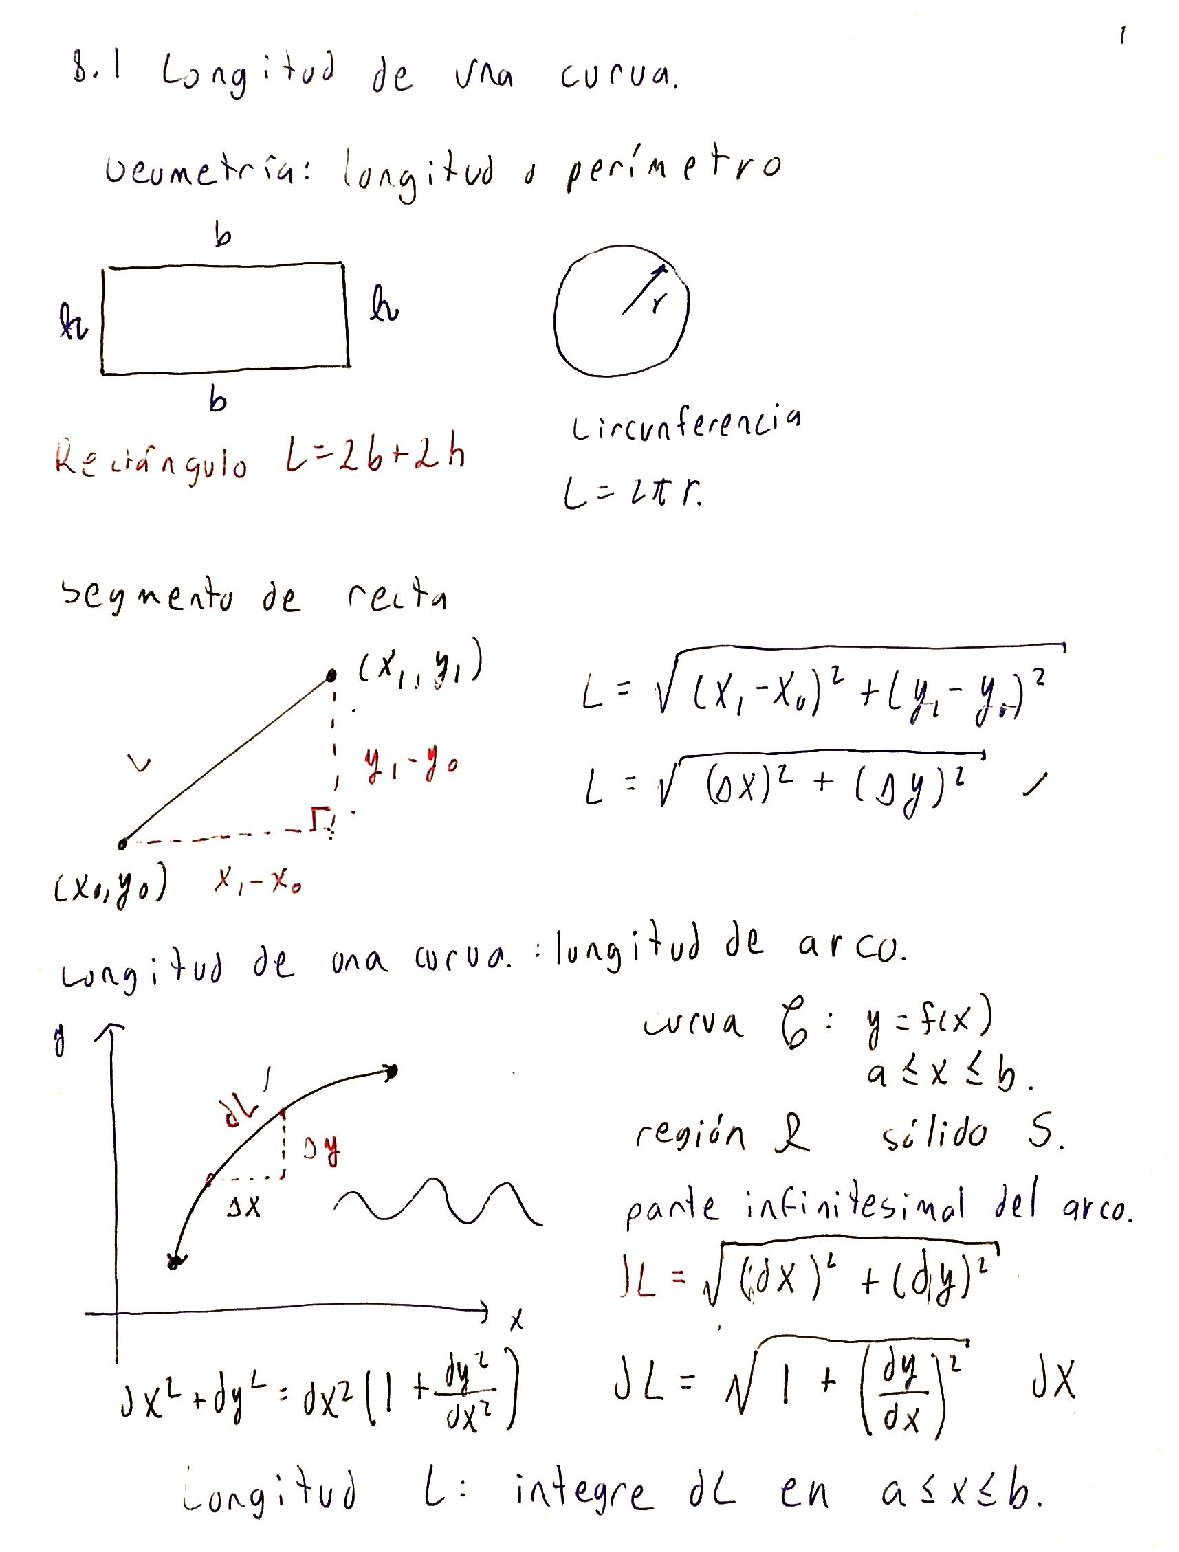
\includepdf[pages=-,pagecommand={\thispagestyle{plain}}]{pdf/RB_2019-09-24_19_01_44.pdf}
%%%%%%%%%%%%%%%%%%%%%%%%%%%%%%%%%%%%%%%%%%%%%%%%%%%%%%%%%%%%%%%%%%%%%%%%%%%%%%%%%%%%%%%%%%%%%%%%

\chapter{8.5 Probabilidad \\ a) Distribución uniforme \\ b) Distribución exponencial \\ c) Distribución normal } 
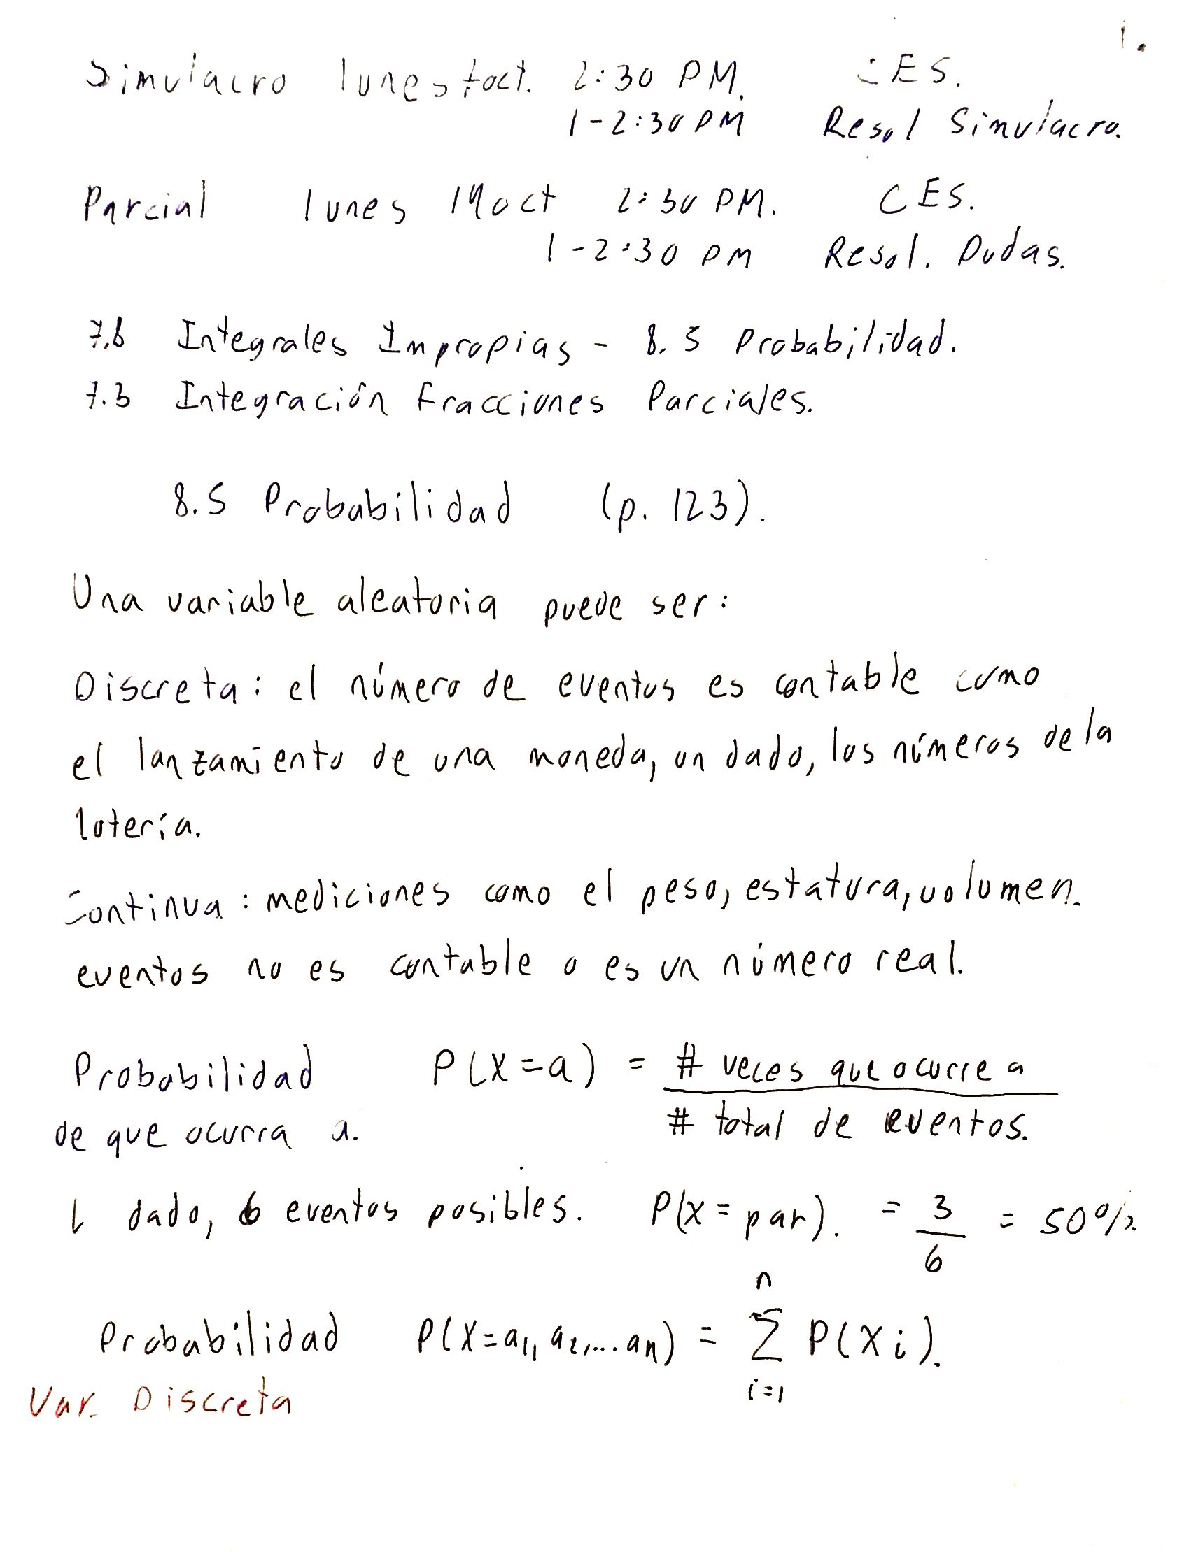
\includepdf[pages=-,pagecommand={\thispagestyle{plain}}]{pdf/RB_2019-09-26_21_38_27.pdf}
%%%%%%%%%%%%%%%%%%%%%%%%%%%%%%%%%%%%%%%%%%%%%%%%%%%%%%%%%%%%%%%%%%%%%%%%%%%%%%%%%%%%%%%%%%%%%%%%

\chapter{8.5 Probabilidad, media, varianza, desviación estándar, mediana } 
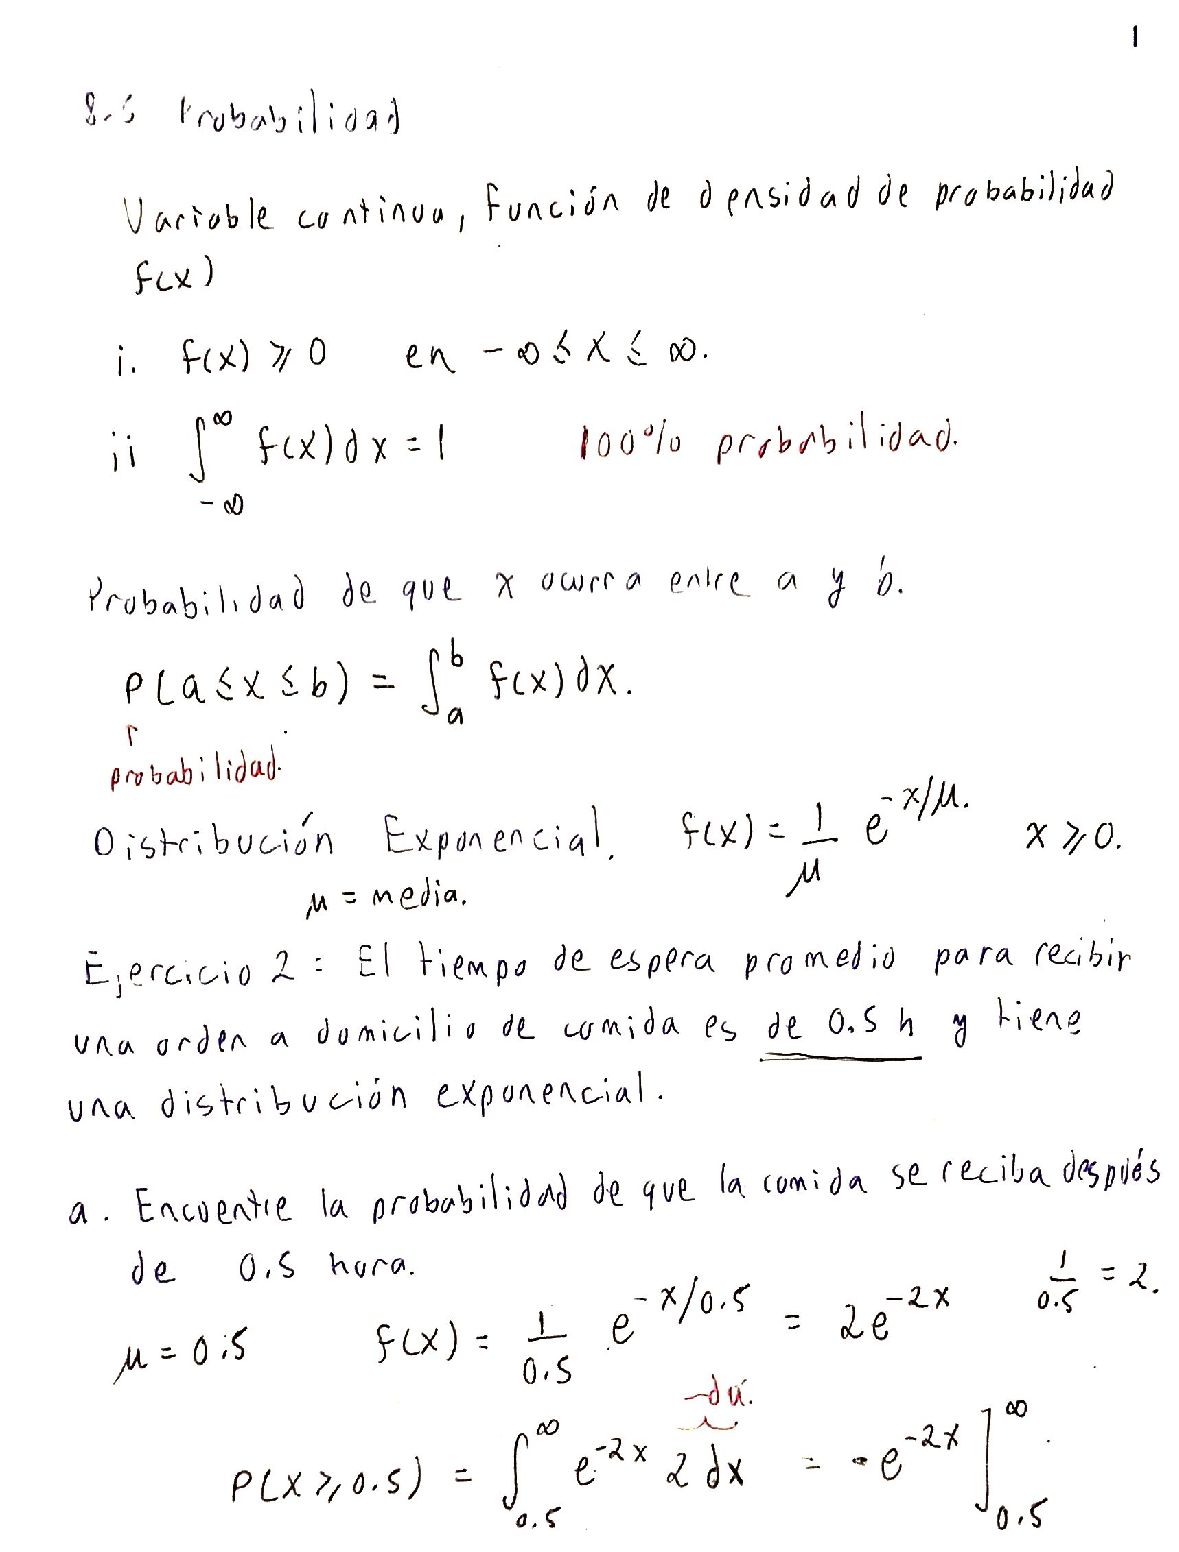
\includepdf[pages=-,pagecommand={\thispagestyle{plain}}]{pdf/RB_2019-10-01_19_28_28.pdf}
%%%%%%%%%%%%%%%%%%%%%%%%%%%%%%%%%%%%%%%%%%%%%%%%%%%%%%%%%%%%%%%%%%%%%%%%%%%%%%%%%%%%%%%%%%%%%%%%

\chapter{7.4 Fracciones parciales \\ Caso 1: Factores lineales distintos \\ Caso 2: Factores lineales repetidos } 
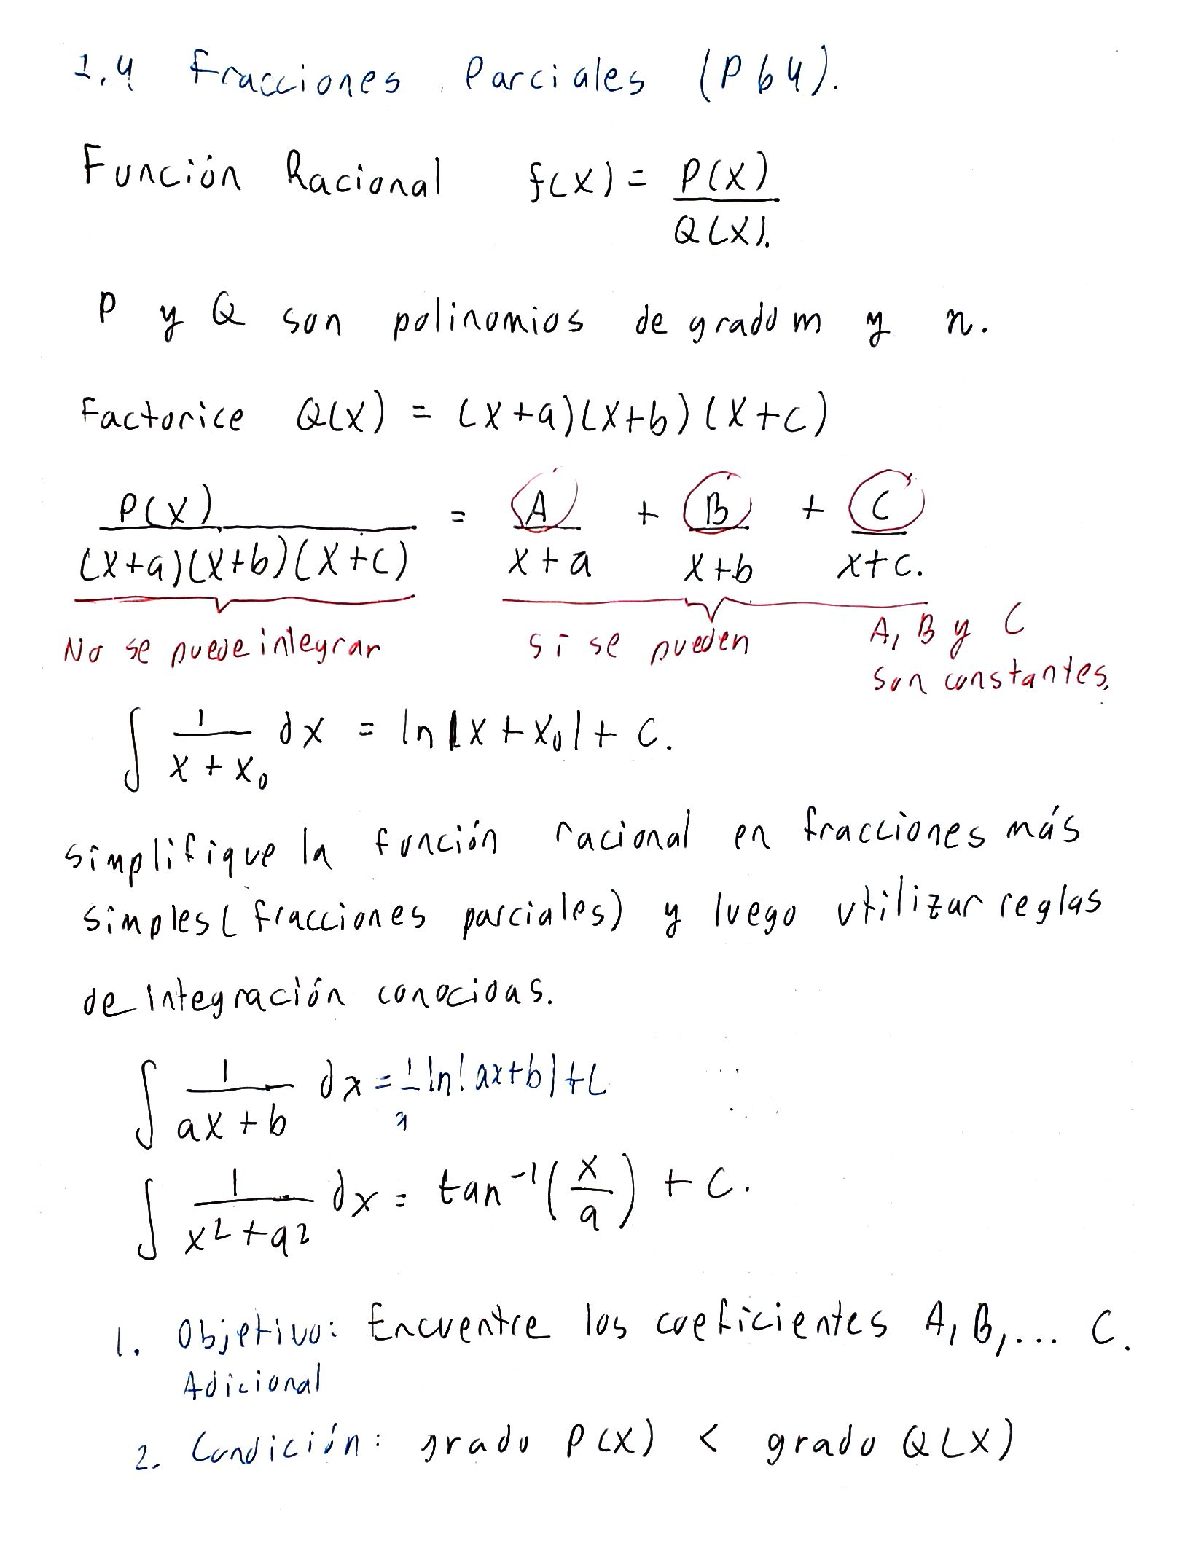
\includepdf[pages=-,pagecommand={\thispagestyle{plain}}]{pdf/RB_2019-10-03_17_17_54.pdf}

%%%%%%%%%%%%%%%%%%%%%%%%%%%%%%%%%%%%%%%%%%%%%%%%%%%%%%%%%%%%%%%%%%%%%%%%%%%%%%%%%%%%%%%%%%%%%%%%

\chapter{7.4 Fracciones parciales \\ Caso 3: Factores cuadráticos irreducibles \\ Caso 4: Factores cuadráticos repetidos } 
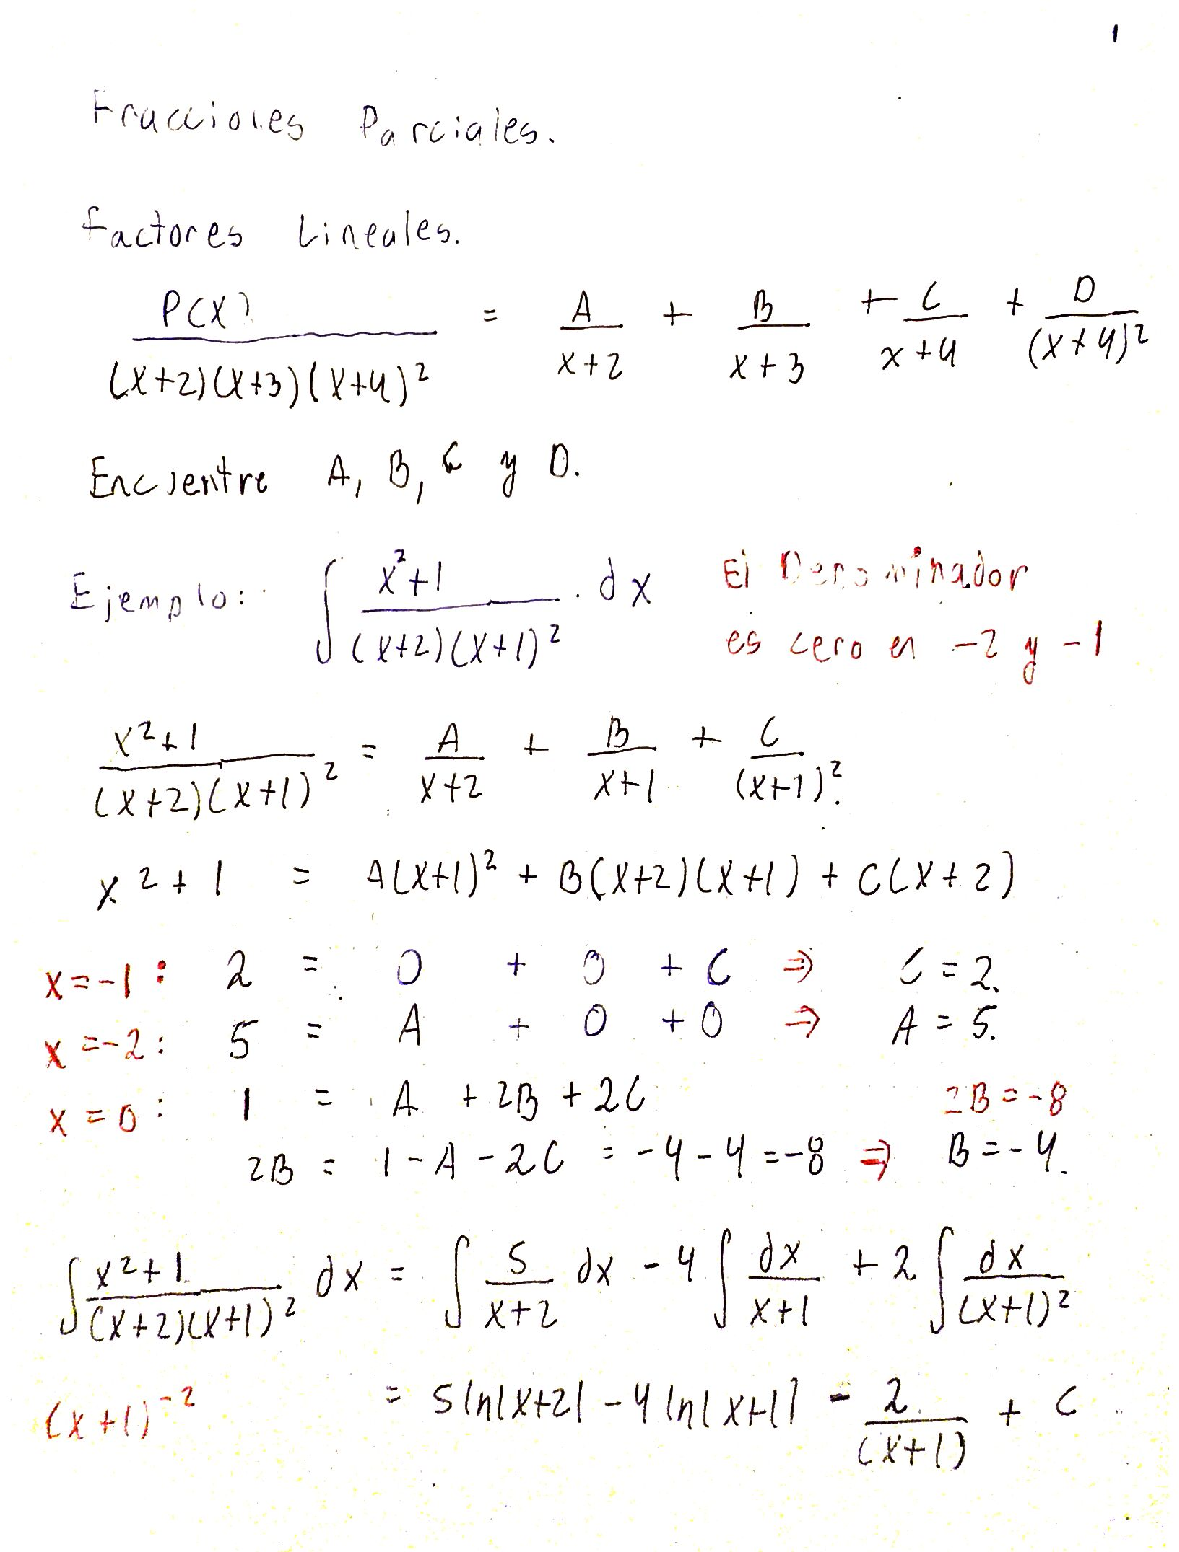
\includepdf[pages=-,pagecommand={\thispagestyle{plain}}]{pdf/RB_2019-10-08_21_15_48.pdf}



\end{document}
